% ----------------------------------------------------------------------------------------------------- %
% Arquivo LaTeX de exemplo de TCC a ser apresentados à Ciência da Computação da UFT - Palmas
% 
% Versão 1.1:   Março 2016
%
% Criado por:   Tiago da Silva Almeida
% Revisado por: Tiago da Silva Almeida
%               Rafael Lima de Carvalho
%               Ary Henrique Morais de Oliveira
%
% http://uftex.sourceforge.net 
% ----------------------------------------------------------------------------------------------------- %

\documentclass[tcc1]{uftex}

\usepackage[num]{abntex2cite}                    % Citações padrão ABNT
% Define os textos da citação
\renewcommand*{\backrefalt}[4]{}%

\makelosymbols
\makeloabbreviations

\usepackage{tikz}                              
\usepackage{verbatim}                      
% Comando para escolha de pacote.
\usepackage{amsmath}
\usepackage[american]{circuitikz}
\usepackage{amsmath,amssymb}
\usepackage{multirow}
\usepackage{listings}
\usepackage{hyperref}
%\usepackage[table,xcdraw]{xcolor} 
\begin{document}
  \title{Avaliação do aprendizado dos acadêmicos da disciplina de Álgebra Linear utilizando o \textit{software} AlfaGebra - módulos sistemas de equações lineares e espaço vetorial.}
  \foreigntitle{Thesis Title}
  \author{Osmir}{Custódio Mariano}
  
  \advisor{Profa.}{Hellena}{Christina Fernandes Apolinário}{Drª.}
  \advisor{Prof.}{Edeilson}{Milhomem da Silva}{Dr.}
  
  \begin{comment}
  \examiner{Prof.}{Nome do Primeiro Examinador Sobrenome}{D.Sc.}
  \examiner{Prof.}{Nome do Segundo Examinador Sobrenome}{Ph.D.}
  \examiner{Prof.}{Nome do Terceiro Examinador Sobrenome}{D.Sc.}
  \end{comment}
  
  \department{CC}
  \date{12}{2017}

  \keyword{Álgebra Linear}
  \keyword{Sistemas lineares}
  \keyword{Espaço vetorial}
  \keyword{Ensino e aprendizagem}

  \foreignkeyword{Linear Algebra}
  \foreignkeyword{Linear systems}
  \foreignkeyword{Vector space}
  \foreignkeyword{Teaching and learning}

  \maketitle

 \frontmatter
 \dedication{Dedico este trabalho aos meus pais, Orlando Mariano da Silva e Maria Gorete Ramos Custódio, que não mediram esforços para que eu chegasse até aqui.}

  \begin{acknowledgement}
  Gostaria de agradecer em primeira lugar a Deus, por possibilitar-me a oportunidade de chegar até aqui, concedendo sabedoria e saúde nessa jornada de 4 (quatro) anos de estudos.
  
  Aos meus pais pelo o apoio deste o momento que recebi a notícia da aprovação no vestibular, aos quais incentivando e aconselhando, e também pelos os esforços realizados para que eu pudesse chegar até nessa etapa de minha vida.
  
  Agradeço a minha orientadora, a professora Dr.ª Hellena Cristina Fernandes Apolinário, pelos ensinamentos, correções, incentivos e atenção para o desenvolvimento deste trabalho, sempre me motivando que irá dar tudo certo nessa jornada de dois semestres.
  
  Agradeço também ao meu coorientador o professor Dr. Edeilson Milhomem da Silva, por aceitar participar deste projeto e pelos seus ensinamentos.
  
  E agradeço aos meus amigos que ajudaram de forma indireta e direta no decorrer do desenvolvimento desse projeto, com revisões e dicas sobre a escrita.
  
  \end{acknowledgement}

\begin{abstract}
    O presente trabalho visa o desenvolvimento de uma plataforma de ensino e aprendizagem AlfaGebra para à disciplina de Álgebra Linear, sendo composta por três módulos: sistemas de equações lineares, espaços vetoriais e transformações lineares, ao qual este estudo abordará o desenvolvimento somente dos módulos de sistemas de equações lineares e espaço vetorial. Cada módulo apresentará conceitos teóricos, exercícios resolvidos e opção para que o usuário possa interagir com a plataforma e assim o sistema será capaz de realizar os cálculos e mostrar o passo a passo da resolução. O desenvolvimento da plataforma abordará a técnica de engenharia de \textit{software}, sendo composta por análise de requisitos, implementação, testes e implantação e será abordada a metodologia de desenvolvimento ágil \textit{Scrum} como procedimento para concretização dos requisitos. Desse modo, o sistema tem como objetivo auxiliar os acadêmicos da disciplina Álgebra Linear no aprendizado dos conteúdos e a partir do mesmo avaliar os discentes através da comparação de uma turma que utilizou a plataforma AlfaGebra e outra que não a utilizou. A avaliação será realizada com aplicação de questionários juntos aos acadêmicos, sendo um questionário aplicado junto a turna que não utilizou o sistema no decorrer do semestre 2017-1 e outro com a turma que utilizará o \textit{software} no decorrer do semestre 2017-2, para assim identificar se houve melhora no aprendizado dos discentes a partir do sistema.
\end{abstract}
  
\begin{foreignabstract}
    The present work aims at the development of an AlfaGebra teaching and learning platform for the discipline of Linear Algebra, being composed of three modules: systems of linear equations, vector spaces and linear transformations, to which this study will address the development of only the systems modules linear equations and vector space. Each module will present theoretical concepts, solved exercises and option so that the user can interact with the platform and thus the system will be able to perform the calculations and show step by step of the resolution. The development of the platform will approach the software engineering technique, consisting of requirements analysis, implementation, testing and deployment, and the agile Scrum development methodology will be approached as a procedure to fulfill the requirements. Thus, the system aims to help students of Algebra Linear in the learning of content and from the same evaluate the students by comparing a group that used the AlfaGebra platform and another that did not use it. The evaluation will be carried out with the application of questionnaires together with the academics, being a questionnaire applied at the turn that did not use the system in the course of the 2017-1 semester and another with the class that will use the software during the 2017-2 semester. identify if there was improvement in the students' learning from the system.
\end{foreignabstract}


\printlosymbols  
\printloabbreviations
\listoffigures            
\listoftables 
\tableofcontents 

\mainmatter
\renewcommand{\baselinestretch}{1.50}\normalsize

% ----------------------------------------------------------------------------------------------------- %
% Capítulos do trabalho
% ----------------------------------------------------------------------------------------------------- %

% ----------------------------------------------------------------------------------------------------- %
% Capítulo 1 - INTRODUÇÃO
% ----------------------------------------------------------------------------------------------------- %
\chapter{Introdução}
\label{cap:introducao}

\noindent A importância da Álgebra Linear tem crescido nas últimas décadas, principalmente nos modelos matemáticos lineares que surgem em diversas áreas, como a economia, aviação, exploração petrolífera, circuitos eletrônicos, estatística, dentre várias outras, e comumente nestes modelos aparecem a resolução de Sistemas de Equações Lineares, a qual de acordo com Leon \cite{1998:Leon} "mais de 75\% de todos os problemas matemáticos encontrados em aplicações científicas e industriais envolvem a resolução de um sistema linear em alguma etapa".  

Para Ana \cite{2010:furtado}, a Álgebra Linear é vista como uma disciplina de fundamental importância para vários estudiosos, como matemáticos e cientistas que a utilizam como instrumento para resoluções de problemas. Dessarte, não é diferente que ela ``constitui uma parte importante no conteúdo matemático que é usado no início de um curso da área de exata". (\cite{1998:dirier}, apud \cite{2010:furtado}, 2010, p. 2).

Na computação gráfica, a aplicação de espaço vetorial é bastante utilizada, em que o espaço espectral de cores é um espaço vetorial de dimensão três, que são as três cores primárias, vermelho, verde e azul, este sistema é conhecido como sistema RGB (\textit{Red, Green} e \textit{Blue}).  Diferentes sistemas de coordenadas, conhecidos como sistemas de cores, são considerados neste espaço vetorial de acordo com a aplicação ou dispositivo de saída gráfica (monitor, impressora, projetor de vídeo, etc.).

Em relação ao ensino e aprendizagem da Álgebra Linear, Celestino \cite{2000:celestino} destaca a importância de pesquisas voltadas para esse estudo:

\begin{quote}
    pesquisas sobre o ensino-aprendizagem da Álgebra Linear repousa no fato de que ela hoje se encontra subjacente a quase todos os domínios da Matemática. Desta forma, é imprescindível que aqueles que pretendem trabalhar com as ciências que utilizam a Matemática, tanto como objeto de seu estudo quanto como instrumento para outros estudos, dominem seus principais conceitos. Por isso se implantou o ensino de Álgebra Linear nos diferentes cursos das chamadas Ciências Exatas, como Engenharia, Física, Química, Ciências da Computação e outras, além de Matemática (p. 9).
\end{quote}

Na Universidade Federal do Tocantins, a disciplina de Álgebra Linear faz parte da estrutura curricular dos cursos de engenharias (Civil, Elétrica, Alimentos e Biotecnológica), Ciência da Computação e Matemática. A citada disciplina é considerada por muitos alunos como difícil, o que é perceptível pelos os altos índices de reprovações e evasão dos acadêmicos. Usando como base a turma do semestre de 2015-1 de Ciência da Computação, de um total de 38 alunos somente 6 passaram com média considerada pela instituição para obter aprovação, sendo superior ou igual a 7 e muitos deles já desistem logo após a aplicação da primeira prova da disciplina.  

Desse modo, a proposta desse trabalho visa o desenvolvimento de uma plataforma de ensino e aprendizagem para a disciplina de Álgebra Linear, com objetivo de auxiliar os acadêmicos no aprendizado dos conteúdos e a partir da plataforma realizar comparação com os estudantes que cursaram a disciplina sem a utilização do \textit{software} e outra com a utilização, para que assim possa avaliar se houve melhora do aprendizado dos estudantes.

\section{Justificativa}

\noindent Nos dias atuais, na era da tecnologia, ainda existem muitos cientistas, matemáticos e engenheiros que dispõem de grande parte do seu tempo realizando pesquisas e muitos deles fazendo cálculos matemáticos manualmente. Devido a era tecnológica, muitos desses cálculos podem serem realizados com auxílios de \textit{software}, dentre alguns deles presente no mercados são: \textit{MatLab, Mathematica, Geogebra} entre outros. A partir da utilização das ferramentas de tecnologias (TICs), possibilita que as tarefas que antes era tediosas para seu desenvolvimento agora elas se tornam mais fáceis de serem desenvolvidas.

Lima \cite{2000:lima} destaca que no atual momento, os computadores se tornaram indispensáveis ao trabalho, como nas áreas da Ciência e Engenharia. E a situação nas instituições acadêmicas não é diferente, em que a cada momento as instituições estão inteiradas acerca da importância do uso de computadores como ferramenta para o ensino e aprendizagem e para isto, elas tem promovido que os acadêmicos ainda na graduação possam ter o contato direto com essas ferramentas para assim auxiliar no aprendizado.

A Álgebra Linear é apresentada como uma área que exige muito esforço no decorrer do aprendizado, visto que é considerada por muitos alunos como uma área difícil de compreender e esse assunto é tão pertinente que alguns pesquisadores já estudaram o desempenho dos acadêmicos que cursam essa disciplina na graduação. Celestino \cite{2000:celestino} em sua pesquisa de mestrado analisou os resultados de reprovações na Universidade Estadual Paulista (UNESP) e Universidade de São Paulo (USP) e identificou que as reprovações giram em torno de 25\% a 50\% e também identificou que pesquisas realizadas em outros países mostraram as dificuldades dos alunos na compreensão dos principais conceitos da Álgebra Linear.

Diante das informações supracitadas e com objetivo de auxiliar os acadêmicos no aprendizado da disciplina de Álgebra Linear do curso de Ciência da Computação, torna primordial o desenvolvimento de uma plataforma de ensino e aprendizagem que ajude a melhor os índices de reprovações e evasão dos estudante da citada disciplina e em conjunto verificar se a plataforma irá realmente auxiliar no processo de aprendizagem, para tal, será realizada uma comparação entre duas turmas de Álgebra Linear, uma que não utilizará \textit{software} e outra que utilizará no decorrer da ministração da disciplina pelo o professor.  

\section{Objetivos}

\subsection{Objetivo Geral}

\noindent O principal objetivo deste trabalho consiste em desenvolver a plataforma de ensino de aprendizagem AlfaGebra e avaliar o aprendizado dos acadêmicos da disciplina de Álgebra Linear do curso de Ciência da Computação.

\subsection{Objetivos Específicos}

Os objetivos específicos são descritos como:

\begin{enumerate}
    \item Desenvolver os módulos de sistemas de equações lineares e espaço vetorial da plataforma AlfaGebra em versão \textit{desktop} para o sistema operacional Windows.
	
	\item Aplicar a metodologia ágil de desenvolvimento iterativo e incremental de \textit{software Scrum}.
	
	\item Comparar o nível de aprendizado dos acadêmicos da disciplina de Álgebra Linear com e sem a utilização do \textit{software} AlfaGebra.
	
	\item Aplicar o teste de usabilidade a fim de um melhor atendimento ao usuário.
\end{enumerate}

\section{Estrutura do Trabalho}

\noindent O Capítulo \ref{cap:algebra} aborda o histórico da Álgebra Linear no geral e a Álgebra Linear na Universidade Federal do Tocantins. Posteriormente, no Capítulo \ref{cap:teoria} é apresentada a fundamentação teórica utilizada no trabalho que é de grande importância para o entendimento desse trabalho. O Capítulo \ref{cap:trabalhos} apresenta os trabalhos relacionados, com destaque em aplicações utilizadas para auxiliar no ensino e aprendizagem. Já no Capítulo \ref{cap:metodologia} é apresentado todo o passo a passo do desenvolvimento desse trabalho e os métodos aplicados para o alcance dos resultados. No Capítulo \ref{cap:resultados} estão apresentados os resultados parciais e por fim, no Capítulo \ref{cap:conclusoes} são descritas as conclusões.

% ----------------------------------------------------------------------------------------------------- %
% Capítulo 2 - ÁLGEBRA LINEAR NA UFT
% ----------------------------------------------------------------------------------------------------- %
\chapter{Ensino da Álgebra Linear}
\label{cap:algebra}

\noindent No decorrer desse capítulo é apresentado um breve histórico sobre a Álgebra Linear e sobre o ensino da Álgebra Linear da Universidade Federal do Tocantins e em especial no curso de Ciência da Computação.

\section{Histórico da Álgebra Linear}

\noindent A Álgebra Linear começou a dar seus primeiros passos no final do século XIX. Com o emergir dos números complexos surgiu a necessidade de relacionar a Álgebra Linear com a Geometria o que nesse contexto, Rodrigues \cite{2009:Rodrigues} explana porque essa necessidade era válida, e isso era devido a aceitação que os números complexos possibilitou na representação geométrica e pelos os testes de representá-los em três dimensões. A partir disso, motivou Willian Rowan Hamilton\footnote[1]{Willian Rowan Hamilton foi um matemático, astrônomo e físico e realizou grandes contribuições no campo da óptica, dinâmica e álgebra.} a constatar os quatérnios, que com eles possibilitou a criação de um sistema, em que a operação de multiplicação não dispunha das propriedades comutativas. E foi nesse ponto que os primeiros passos da Álgebra Linear começaram rumo à sua criação.

Com o surgimento da Álgebra Linear, alguns trabalhos foram desenvolvidos a fim de demonstrar esse novo ramo da matemática e dentre os trabalhos de grande destaque sobre esse estudo encontra-se nos Estados Unidos e na França com início de sua criação nos anos 80. Furtado \cite{2011:Furtado} relata que um grupo de pesquisadores na França desenvolveu um conjunto de artigos a respeito da Álgebra Linear e que logo após tornaram-se um livro, intitulado de \textit{L'Enseignement de L'Algébre Linéaire en Question} \cite{1998:dirier}, coordenado pelo o autor de maior destaque na área, Dorier. Em relação aos trabalhos desenvolvidos nos Estados Unidos, a revisão do currículo da Álgebra Linear foi realizada e então surgiu o grupo de estudo \textit{Linear Algebra Curriculum Study Group} (LACSG), sendo orientado por David Carlson. 

Dez anos depois da primeira publicação de artigos a respeito do tema Álgebra Linear, a \textit{Mathematical Association of America} (MAA) começou a formação \textit{Algebra Curriculum Study Group} (LACSG). E não demorou muito para o LACSG concluir o primeiro curso de Álgebra Linear em um curso de engenharia. No primeiro curso alguns requisitos foram aplicados, tais como a utilização de ferramentas tecnológicas para melhor aproveitamento do ensino.

O estudo da Álgebra Linear no Brasil começou a se desenvolver nos anos 90 e de acordo com Ana \cite{2010:furtado}, até 2010 no Brasil a produção de trabalhos voltados para Álgebra Linear eram poucos e a pesquisadora que mais desenvolveu pesquisas na área foi Marlene Alves Dias, que começou a trabalhar em suas produções na França. Celestino \cite{2000:celestino} desenvolveu sua dissertação de Mestrado em que estudava o histórico do ensino e aprendizagem da Álgebra Linear, ao qual focou nos poucos trabalhos que existiam no atual momento e também citou de outros países.

Alguns matemáticos realizaram grande contribuição para a evolução da Álgebra Linear entre eles Lagrange (1736-1813), Frobenius (1849-1917), Hamilton(1805-1865), Gauss (1777-1855), entre outras.

\section{Álgebra Linear na UFT}

\noindent A Universidade Federal do Tocantins (UFT) apresenta em seu catálogo cursos em diversas áreas, tais como: saúde, meio ambiente, tecnologia da informação, engenharia, entre outros e dentre essas áreas existem a presença dos cursos que dispõem em sua estrutura curricular disciplinas matemáticas e em especial a de Álgebra Linear, como as engenharias (Civil, Elétrica, Alimentos, e Biotecnológica), matemática e Ciência da Computação.

Na maioria dos cursos a disciplina de Álgebra Linear é ofertada no terceiro período e semestralmente são atendidos aproximadamente 280 (duzentos e oitenta) alunos em todos os \textit{campi}. Em relação a estrutura curricular em cada curso apresenta uma pequena variação, mas todos dispõem dos conteúdos de sistemas de equações lineares, espaço vetorial e transformações lineares.

\subsection{Álgebra Linear no curso de Ciência da Computação}

\noindent O curso de Ciência da Computação na Universidade Federal do Tocantins, apresenta em sua estrutura curricular a disciplina de Álgebra Linear, a qual é ofertada no terceiro período e apresenta como objetivo introduzir os conceitos fundamentais da Álgebra Linear e assim os acadêmicos possam adquirir conhecimentos e aplicá-los para resoluções de problemas ligados a computação, por exemplo, à computação gráfica que aborda muitos dos conceitos e implementação utilizadas na Álgebra Linear.

A disciplina se desenvolve em um semestre, com carga horária de 60h, sem a exigência de pré-requisitos e apresenta como conteúdos principais sistemas de equações lineares, espaço vetorial e transformações lineares.

Semestralmente a coordenação do curso de Ciência da Computação ofertam 40 vagas e na grande maioria todas são preenchidas, contudo nem todos os alunos concluem à disciplina o que é demostrado pelos índices de desistências que são elevados, na qual, considerando a turma do período de 2015-2 de um total de 38 alunos, 21 desses desistem da disciplina logo após a aplicação da primeira avaliação ou até mesmo antes e esses dados correspondem a mais da metade da turma com 55,28\% e é importante destacar que na grande maioria dos períodos a quantidade de alunos que são evadidos esse índice é alto.
% ----------------------------------------------------------------------------------------------------- %
% Capítulo 3 - FUNDAMENTAÇÃO TEÓRICA
% ----------------------------------------------------------------------------------------------------- %
\chapter{Fundamentação Teórica}
\label{cap:teoria}

\noindent Ao longo desse capítulo serão expostos conceitos básicos que são de grande importância para o entendimento desse trabalho e dentre eles serão destacados a definição de matriz e uma explanação sobre as principais utilizadas no estudo da Álgebra Linear, sistemas de equações lineares que são uns dos conteúdos que farão parte da plataforma de ensino e aprendizagem AlfaGebra, espaço vetorial que também compõe o AlfaGebra, abordagem sobre engenharia de \textit{software} a fim de explanar como consiste o desenvolvimento de um sistema, e para um desenvolvimento mais enxuto a utilização da metodologia ágil \textit{Scrum} que será aplicada no desenvolvimento do \textit{software} AlfaGebra e assim entender seu funcionamento. E por fim, uma abordagem sobre avaliação do ensino e aprendizagem.

\section{Matrizes}
\noindent Um das ferramentas mais poderosas consideradas na matemática são as matrizes, pois as mesmas tem aplicações em diversas áreas, tais como em codificação e decodificação de mensagens, computação gráfica, engenharias, etc. Desse modo, faz-se necessário a compreensão de algumas propriedades e nomenclaturas em relação as mesmas.

\subsection{Definição de matriz}
\noindent Matrizes são objetos matemáticos estruturados em um quadrado composto por linhas e colunas. A definição de Steinbruch \cite{1987:Steinbruch} é similar a citada, onde uma matriz é um quadrado $m x n$ de elementos, e que estes podem ser números, polinômios, funções, etc., que estão dispostos em $m$ linhas e $n$ colunas, representada por  $A{}_{mxn}$.\\

\begin{center}
    $A = 
    \begin{bmatrix}
        a_{11} & a_{12} & a_{13} & \ldots & a_{1n}\\ 
        a_{21} & a_{22} & a_{23} & \ldots & a_{2n}\\ 
        a_{31} & a_{32} & a_{33} & \ldots & a_{3n}\\ 
        \vdots & \vdots & \vdots & \ldots & \\ 
        a_{m1} & a_{m2} & a_{m3} & \ldots & a_{mn}
    \end{bmatrix}_{mxn}$
\end{center}

%
\subsection{Tipos de matrizes}
\noindent Para Boldrini \cite{1980:Boldrini}, no processo de utilização de matrizes, percebe-se que existem algumas que são diferentes, seja pela quantitativo de linhas ou colunas, bem como também pela natureza de seus elementos, a qual apresentam propriedades que se diferenciam de uma matriz qualquer. A seguir, serão expostas as principais categorias de matrizes, para isso, considerando uma matriz com $m$ linhas e $n$ colunas representa por $A{}_{mxn}$.

\subsubsection{Matriz Quadrada}
\noindent Quando o número de linhas $m$ é igual ao número de coluna $n$ $(m = n)$.

\textit{Exemplo:}
\begin{center}
    $A = 
    \begin{bmatrix}
        a_{11} & a_{12} & a_{13} \\ 
        a_{21} & a_{22} & a_{23} \\ 
        a_{31} & a_{32} & a_{33} 
    \end{bmatrix}_{mxn}$
\end{center}

Observando a matriz $A$, percebe-se que o número de linhas e colunas são iguais, sendo $A{}_{3x3}$. Nesse tipo de matriz, em que a ordem é $n$ por $n$, costuma dizer que $A$ é uma matriz de ordem $n$.

\subsubsection{Matriz Linha}
\noindent A matriz que apresenta somente uma linha, ou seja, matriz de ordem $1$ por $n$.

\textit{Exemplo:}
\begin{center}
    $A = 
    \begin{bmatrix}
        a_{1} & a_{2} & a_{3} & \ldots & a_{n}
    \end{bmatrix}_{n x 1}$
\end{center}

\subsubsection{Matriz Coluna}
\noindent A matriz que apresenta somente uma coluna, ou seja, matriz de ordem $n$ por $1$.

\textit{Exemplo:}
\begin{center}
    $A = 
    \begin{bmatrix}
        a_{1} \\ 
        a_{2} \\
        a_{3} \\
        \vdots \\
        a_{n} 
    \end{bmatrix}_{1 x n}$
\end{center}

\subsubsection{Matriz Nula}
\noindent A matriz cujos elementos $a{}_{mn}$ são todos nulos.

\textit{Exemplo:}
\begin{center}
    $A = 
    \begin{bmatrix}
        0 & 0 & 0\\ 
        0 & 0 & 0 
    \end{bmatrix}$
\end{center}

\subsubsection{Matriz Diagonal}
\noindent É uma matriz quadrada em que os elementos que não pertencem a diagonal principal são todos nulos, denotada por $A{}_{mn} = 0$, para $m \neq n$.

\textit{Exemplo:}
\begin{center}
    $A = 
    \begin{bmatrix}
        a_{11} & 0 & 0 \\ 
        0 & a_{22} & 0 \\ 
        0 & 0 & a_{33}  
    \end{bmatrix}$
\end{center}

\subsubsection{Matriz Identidade}
\noindent A matriz escalar de qualquer ordem que tem todos os elementos da diagonal principal $a{}_{mm} = 1$ e $a_{mn} = 0$, para todo $m \neq n$. Representada com $I{}_{n}$, ou simplesmente por $I$ é chamada de matriz identidade.

\textit{Exemplo:}
\begin{center}
    $I_{3} = 
    \begin{bmatrix}
        1 & 0 & 0 \\ 
        0 & 1 & 0 \\ 
        0 & 0 & 1  
    \end{bmatrix}$
\end{center}

\subsection{Operações com matrizes}
\noindent Para uma melhor utilização das matrizes é necessário um entendimento sobre as operações aritméticas aplicadas nelas. Assim, a seguir serão demonstradas as três operações que são aplicadas nelas.

\subsubsection{Multiplicação por um escalar}
\noindent De acordo coma definição de Leon \cite{1998:Leon}, se $A$ é uma matriz e $\alpha$ é um escalar, assim $\alpha A$ será a matriz gerada a partir da multiplicação de cada elemento de $A$ por $\alpha$.

\textit{Exemplo:}
\begin{center}
    $5 x
    \begin{bmatrix}
        1 & 3 & 6 \\ 
        -4 & 2 & 0 \\ 
        5 & 7 & -1  
    \end{bmatrix}
    =
    \begin{bmatrix}
        5 \cdot 1 & 5 \cdot 3 & 5 \cdot 6 \\ 
        5 \cdot (-4) & 5 \cdot 2 & 5 \cdot 0 \\ 
        5 \cdot 5 & 5 \cdot 7 & 5 \cdot (-1)  
    \end{bmatrix}
    =
    \begin{bmatrix}
        5 & 15 & 30 \\ 
        -20 & 10 & 0 \\ 
        25 & 35 & -5
    \end{bmatrix}$
\end{center}

Em relação as propriedades da multiplicação de uma matriz por um escalar, para quaisquer matrizes $A$ e $B$ de mesma ordem e os escalares $\alpha$ e $\lambda$ reais a multiplicação por o escalar satisfaz as presentes propriedades:
\begin{enumerate}
    \item[i)] $(\alpha \lambda) A = \alpha(\lambda A)$
    \item[ii)] $(\alpha + \lambda) A = \alpha A + \lambda A$
    \item[iii)] $\alpha(A + B) = \alpha A + \alpha B)$
    \item[iv)] $1 A = A$
\end{enumerate}
 
\subsubsection{Soma de matrizes}
\noindent Dadas duas matrizes $A = (a{}_{mn})$ e $B = (b{}_{mn}) $ são matrizes $m x n$. Assim, a soma $A + B$ é a matriz $m x n$, cujos elementos $(m, n)$ é $(a{}_{mn}) + (b{}_{mn})$, para cada par ordenado $(m, n)$.

\textit{Exemplo:}
\begin{center}
    $A =
    \begin{bmatrix}
        a{}_{11} & a{}_{12} & a{}_{13} \\ 
        a{}_{21} & a{}_{22} & a{}_{23} 
    \end{bmatrix}
    + B =
    \begin{bmatrix}
        b{}_{11} & b{}_{12} & b{}_{13} \\ 
        b{}_{21} & b{}_{22} & b{}_{23}
    \end{bmatrix}
    =
    \begin{bmatrix}
        a{}_{11} + b{}_{11} & a{}_{12} + b{}_{12} & a{}_{13} + b{}_{13} \\ 
        a{}_{21} + b{}_{21} & a{}_{22} + b{}_{12} & a{}_{23} + b{}_{13}
    \end{bmatrix}$
\end{center}

Em relação às propriedades da adição de matrizes, para quaisquer matrizes $A, B$ e $C$ de mesma ordem $m x n$, existem as seguintes propriedades que a satisfazem:

\begin{enumerate}
    \item[i)] $A + (B + C) = (A + B) + C$
    \item[ii)] $A + 0 = 0 + A = A$
    \item[iii)] $-A + A = A - A = 0$
    \item[iv)] $A + B = B + A$
\end{enumerate}

\subsubsection{Multiplicação de matrizes}
\noindent Uma das operações mais importantes é a multiplicação entre matrizes. De acordo com Leon \cite{1998:Leon}, a motivação da definição a seguir de multiplicação entre matrizes vem de sua aplicação em sistemas lineares.

A definição dada por Leon \cite{1998:Leon}, diz que, se $A = (a{}_{mn})$ é uma matriz $m x n$ e  $B = (b{}_{mn)$ é uma matriz $n x r$, assim o produto $AB = C = (c{}_{mn)$ é a matriz $m x r$ cujos elementos são definidos por 

\begin{center}
    $c_{mnj} = \sum_{i}^{k=1}a_{mk}b_{kn}$
\end{center}

Desse modo, para formar o elemento $(m, n)$ do produto, pega-se a \textit{m-ésima} linha de $A$ e a \textit{n-ésima} coluna de $B$, e assim multiplicam-se os elementos correspondentes dois a dois e soma-se os números resultantes. Contudo, para que o produto $AB$ seja possível é necessário que exista se, e somente se, o número de colunas de $A$ seja igual ao número de linhas $B$.

\textit{Exemplo:}
\begin{center}
    $A = 
    \begin{bmatrix}
        1 & 2 & 3 \\ 
        -2 & 1 & 6 
    \end{bmatrix}$
    e $B = 
    \begin{bmatrix}
        3 & -2 \\ 
        2 & 4 \\
        1 & -3 
    \end{bmatrix}$
\end{center}

então:

\begin{center}
    $AB =
    \begin{bmatrix}
        1 \cdot 3 + 2 \cdot 2 + 3 \cdot 1 & 1 \cdot (-2) + 2 \cdot 4 + 3 \cdot (-3) \\ 
        (-2) \cdot 3 + 1 \cdot 2 + 6 \cdot 1 & (-2) \cdot (-2) + 1 \cdot 4 + 6 \cdot (-3)
    \end{bmatrix}
    =
    \begin{bmatrix}
        10 & -3 \\ 
        2 & -10 
    \end{bmatrix}$
\end{center}

\section{Sistemas de Equações Lineares}
\noindent Na matemática, provavelmente um dos problemas considerados mais importantes é a resolução de sistemas de equações lineares. Leon \cite{1998:Leon} destaca a importância desse conteúdo na Álgebra Linear, visto que muitos dos problemas matemáticos que são encontrados em aplicações científicas e industriais abordam em alguma etapa do processo a resolução de um sistema linear. Usando os métodos matemáticos modernos, em muitos dos casos é possível minimizar o problema a um único sistema de equações lineares. E as aplicações e utilização de sistemas de equações lineares está presente em várias áreas como administração, sociologia, economia, ecologia, demografia, engenharia, física, genética, entre outras.

\subsection{Equação Linear}
\noindent Por definição uma equação linear é uma equação da forma: 
\begin{center}
    $a_{1}x_{1} + a_{2}x_{2} + a_{3}x_{} + ... + a_{n}x_{n} = b$   
\end{center}
onde $a_{1}, a_{2}, ..., a_{n}$ são os coeficientes das variáveis, b o termo independente e $x_{1}, x_{2}, x_{3}, ..., x_{n}$ são variáveis.

\subsection{Sistemas de equações lineares}
\noindent Um sistema de equações lineares refere-se a um conjunto de equações do tipo:\\

$\left\{\begin{matrix}
    a_{11}x_{1} + a_{12}x_{2} + a_{13}x_{3} + \ldots + a_{1n}x_{n} = b_{1}\\ 
    a_{21}x_{1} + a_{22}x_{2} + a_{23}x_{3} + \ldots + a_{2n}x_{n} = b_{2}\\ 
    a_{31}x_{1} + a_{32}x_{2} + a_{33}x_{3} + \ldots + a_{3n}x_{n} = b_{3}\\ 
    \ldots\\ 
    a_{m1}x_{1} + a_{m2}x_{2} + a_{m3}x_{3} + \ldots + a_{mn}x_{n} = b_{m}\\ 
\end{matrix}\right$

\subsection{Operações Elementares}
\noindent As operações elementares sobre as linhas de uma matriz são um total de três:
\begin{itemize}
    \item Permutação de duas equações $(Linha_{m} \rightarrow Linha_{n})$:\\
    \textit{Exemplo:}\\
    $Linha_{2} \rightarrow Linha_{3}$
    $\begin{center}
        \begin{bmatrix}
         a & b\\ 
         c & d\\ 
         e &  f
        \end{bmatrix}
        \rightarrow 
        \begin{bmatrix}
         a & b\\ 
         e & f\\ 
         c & d
        \end{bmatrix}\\
    \end{center}$\\
\end{itemize}

\begin{itemize}
    \item Multiplicação de uma equação por um escalar $k$ não nulo $(Linha_{m} \rightarrow k\cdot Linha_{n})$:\\
    \textit{Exemplo:}\\
    $Linha_{2} \rightarrow 2 \cdot Linha_{2}$
    $\begin{center}
        \begin{bmatrix}
         a & b\\ 
         c & d\\ 
         e &  f
        \end{bmatrix}
        \rightarrow 
        \begin{bmatrix}
         a & b\\ 
         2 \cdot c & 2 \cdot d\\ 
         e & f
        \end{bmatrix}\\
    \end{center}$\\
\end{itemize}

\begin{itemize}
    \item Substituição de uma linha por sua soma com outra equação previamente multiplicada por um escalar $k$ não nulo $(Linha_{i} \rightarrow Linha_{m} + k \cdot Linha_{n})$:\\
    \textit{Exemplo:}\\
    $Linha_{2} \rightarrow Linha_{2} + 2 \cdot Linha_{1}$
    $\begin{center}
        \begin{bmatrix}
         a & b\\ 
         c & d\\ 
         e &  f
        \end{bmatrix}
        \rightarrow 
        \begin{bmatrix}
         a & b\\ 
         c+2 \cdot a & d+2 \cdot b\\ 
         e & f
        \end{bmatrix}$\\
    \end{center}
\end{itemize}

\subsection{Forma Escada}
\noindent Por definição dada por Boldrini \cite{1980:Boldrini}, uma matriz de dimensões $m \times n$ é considerada linha reduzida à forma escada se atender aos presentes requisitos abaixo:

\begin{enumerate}
    \item O primeiro elemento de cada linha diferente de zero é igual a 1.
    \item Cada coluna que apresenta o primeiro elemento diferente de zero de alguma linha tem todos os demais elementos iguais a zero.
    \item Se existirem linhas com todos os elementos iguais a zero, elas ficam abaixo de todas as linhas não-nulas.
    \item O número de zeros que preceda o primeiro elemento não nulo, aumenta a cada linha.
\end{enumerate}

\subsubsection{Definição:}
\noindent Dada uma matriz $A_{mxn}$, seja $B_{mxn}$ a matriz linha reduzida à forma escada de $A$. O posto de $A$, denotado por $P$ é a quantidade de linhas não nulas de $B$ e a nulidade de $A$ é o número $n-p$.

\subsection{Soluções de um sistema de equações lineares}
\noindent Dentro da resolução de sistemas de equações lineares podem ocorrer diversas situações na resolução. Considerando um sistema ax = b existirão três possibilidades:
\begin{enumerate}
    \item O sistema possui uma única solução. O sistema nesse caso é dito compatível e determinado ou sistema possível e determinado.
    \item Sistema possui infinitas soluções. O sistema é dito compatível e indeterminado ou sistema possível e indeterminados.
    \item Sistema não possui solução. O sistema é dito incompatível ou impossível. 
\end{enumerate}

\section{Espaço Vetorial}
\noindent Leon \cite{1998:Leon} explana que ``as operações de soma e multiplicação por um escalar são usadas em diversos contextos em matemática. Independentemente do contexto, no entanto, essas operações obedecem, em geral, ao mesmo conjunto de regras aritméticas". E diante de tal, aplicações de sistemas matemáticos que abordam as operações de soma e multiplicação por um escalar apresentam aplicações em várias áreas da matemática e esses sistemas matemáticos desse modelo são chamados de espaços vetoriais. 

Abramo \cite{2016:Abramo} destaca que espaço vetorial está presente em zonas importantes da análise matemática e da geometria diferencial. A utilização de espaços vetoriais está presente em diversas aplicações e áreas, dentre algumas delas, a computação gráfica com sua utilização no espaço espectral de cores, no sistema RGB (\textit{Red, Green e Blue}), em aplicações na física moderna, entre outras.

\subsection{Espaços Vetoriais}
\subsubsection{Definição}
\noindent Boldrini \cite{1980:Boldrini} defini um espaço vetorial real como um conjunto $V$, não vazio, com as seguintes operações: soma, $V\times V\overset{+}{\rightarrow}V$ e a multiplicação por escalar, $\mathbb{R}\times V\overset{\cdot}{\rightarrow}V$ assim, para quaisquer $u, v, w$ e $a, b \in \mathbb{R}$, as propriedades são satisfeitas.

\subsubsection{Operação soma}
\begin{enumerate}
    \item $(u + v) + w = u + ( v + w)$
    \item $u + v = v + u$
    \item Existe $0 \in v$ tal que $0 + v = v$ (0 é chamado vetor nulo)
    \item Existe $- u \in v$ tal que $u + (-u) = 0$
\end{enumerate}
\subsubsection{Operação multiplicação}
\begin{enumerate}
    \item $a(u + v) = au + av$
    \item $(a + b)v = av + bv$
    \item $(ab)v = a(bv)$
    \item $1u = u$
\end{enumerate}

\subsection{Subespaços Vetoriais}
\noindent Em alguns casos é necessário descobrir dentro de um espaço vetorial $V$, subconjuntos $W$ que sejam eles próprios espaços vetoriais menores. Estes conjuntos são chamados de subespaços de $V$. Por exemplo, considerando $V = R^{2}$ o plano onde $W$ é uma reta deste plano, que passa pela origem.

\begin{figure}[!hb]
  \centering 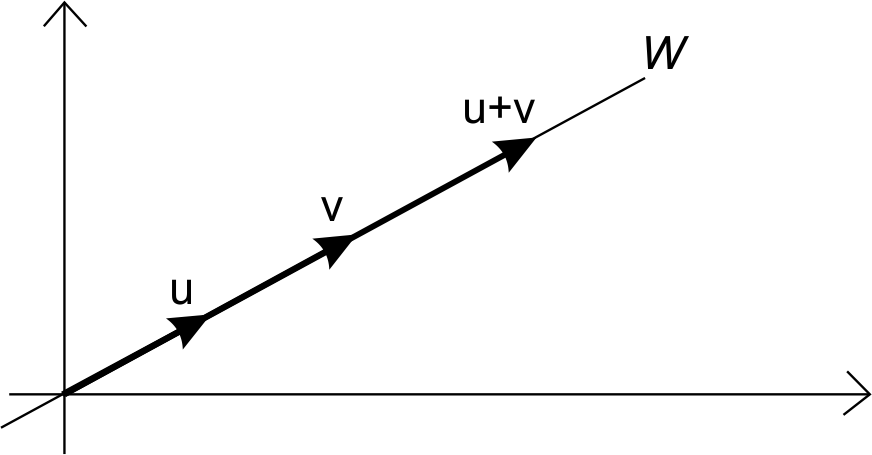
\includegraphics[dimensões]{Figuras/subespacos.png}
  \caption{Subespaço.}
  \label{chave_para_refencia_cruzada}
\end{figure}

\subsubsection{Definição:}
\noindent Dado um espaço vetorial de $V$, um subconjunto $W$, não vazio, será um espaço vetorial de $V$ se atender as duas condições:

\begin{enumerate}
    \item $\forall u, v \in W \rightarrow u + v \in W$
    \item $\forall \alpha \in \mathbb{R}$ e $u \in W \rightarrow \alpha u \in W$
\end{enumerate}

\textit{Exemplo:}\\
Nesse exemplo verifica-se se o conjunto $W = \left \{ (x, 2x) ; x \in \mathbb{R} \right \} \subset \mathbb{R}^2$ é um subespaço vetorial.

Inicialmente deve-se verificar se o vetor nulo está dentro do subespaço assim:
\begin{center}
    $(0, 2\cdot0) = (0,0) \in W$    
\end{center}
Como a verificação é válida, o vetor nulo encontra-se dentro do subespaço, agora analisando as condições da definição:

\subsubsection{Condição 1}
\noindent Sejam $u = (x_{1}, 2x_{1}), v = (x_{2}, 2x_{2}) \in W$. Verificando se $u + v \in W$:
\begin{center}
    $u + v = (x_{1}, 2x_{1}) + (x_{2}, 2x_{2})$\\
    $u + v = (x_{1} + x_{2}, 2x_{1}) + 2x_{2})$\\
    $u + v = (x_{1} + x_{2}, 2(x_{1} + x_{2}) \in W$\\
\end{center}
Observando o resultado obtido percebe-se que a ordenada é o dobro da abscissa.

\subsubsection{Condição 2}
\noindent Sejam $\alpha \in \mathbb{R}$ e $u = (x_{1}, 2x_{1}) \in W$. Verificando se $\alpha u \in W$:
\begin{center}
    $\alpha u = \alpha(x_{1}, 2x_{1})$\\
    $\alpha u = (\alpha x_{1}, \alpha 2x_{1})$\\
    $\alpha u = (\alpha x_{1}, 2(\alpha x_{1})) \in W$\\
\end{center}
Como as duas condições são satisfeitas, então o conjunto é um subespaço vetorial.


\subsection{Computação simbólica}
\noindent A computação simbólica ou como é conhecida também, computação algébrica, é uma área da computação que trata do estudo e desenvolvimento de algoritmos para manipulação de expressões matemáticas e outros objetos matemáticos. Campos \cite{2015:Lidio} define a computação simbólica como:
\begin{quote}
    um interessante recurso de programação de alto nível, que integra os paradigmas de programação procedural, programação funcional e programação baseada em regras, que permite aos programadores especialistas produzirem aplicações que sistematicamente trabalham o desenvolvimento de Cálculo analítico avançado (p. 4).  
\end{quote}
A computação simbólica é bastante utilizada na matemática para o desenho de fórmulas que são utilizadas em programas numéricos e esse recurso que ele possibilita ajuda a simplificar as tarefas dos usuários ao realizarem cálculos manualmente.

\section{Metodologia de Desenvolvimento Ágil}
\noindent Um ponto importante das metodologias ágeis é que elas são adaptativas, ou seja, elas podem ser adaptadas no decorrer do desenvolvimento de \textit{software} a novos fatores, o que é diferente das metodologias clássicas, a qual pode acontecer de no decorrer do desenvolvimento de um \textit{software} realizar todas as etapas necessárias para sua concretização e depois verificar que elas não atendem mais ao propósito que foi implementado. Isso porque as regras podem ter mudado e para a realização das adaptações pode ter um custo alto, desse modo, não sendo proveitoso desenvolvê-las. Foi a partir dessa situação que a crise do \textit{software} começou a crescer, visto que os \textit{software} não satisfaziam os clientes ou empresas \cite{2005:rezende}.

\subsection{Manifesto Ágil}
\noindent O manifesto ágil teve seu surgimento em 2001 pelo engenheiro de \textit{software} Kenet Beck e mais 16 (dezesseis) desenvolvedores de sistemas de grande destaques na área, a qual batizaram de \textit{"Agile Alliance"} e assinaram um documento conhecido com \textit{"Manifesto para Desenvolvimento Ágil de \textit{Software}"} como registro dessa prática de desenvolvimento \cite{2001:Pressman}.

Atualmente o processo de desenvolvimento de \textit{software} utilizando a metodologia ágil tem ganhado bastante espaços devido ao fato que Pereira \cite{2013:Pereira} relata:
\begin{quote}
    os processos ágeis de desenvolvimento compartilham a premissa de que o cliente aprende sobre as suas necessidades, na medida em que é capaz de manipular o sistema que está sendo produzido e, com base no \textit{feedback} do sistema, ele reavalia as suas necessidades e prioridades, criando mudanças que devem ser incorporadas ao \textit{software} (\cite{2013:Pereira}, apud \cite{2004:Teles}, 2004). 
\end{quote}

\subsection{Metodologia \textit{Scrum}}
\noindent Dentre as metodologias ágeis atualmente presentes no mercado, existe o \textit{Scrum}, esta criada em 1990 por Jeff Sutherland e sua equipe de desenvolvimento, mas somente na década seguinte que se tornou popular. Recentemente Scwaber Beedle foi o responsável por adicionar novas atualizações na metodologia \cite{2001:Pressman}. Tal metodologia aborda todos os princípios utilizados pelo o manifesto ágil, visando a orientação sobre o desenvolvimento de \textit{software} nas atividades de requisitos como levantamento e análise de requisitos, planejamento do projeto, evolução e entrega do produto são atendidos.

O \textit{Scrum} funciona de acordo com seu ciclo de atividades como a figura \ref{chave_para_refencia_cruzada} é demonstrada.

\begin{figure}[!hb]
  \centering 
  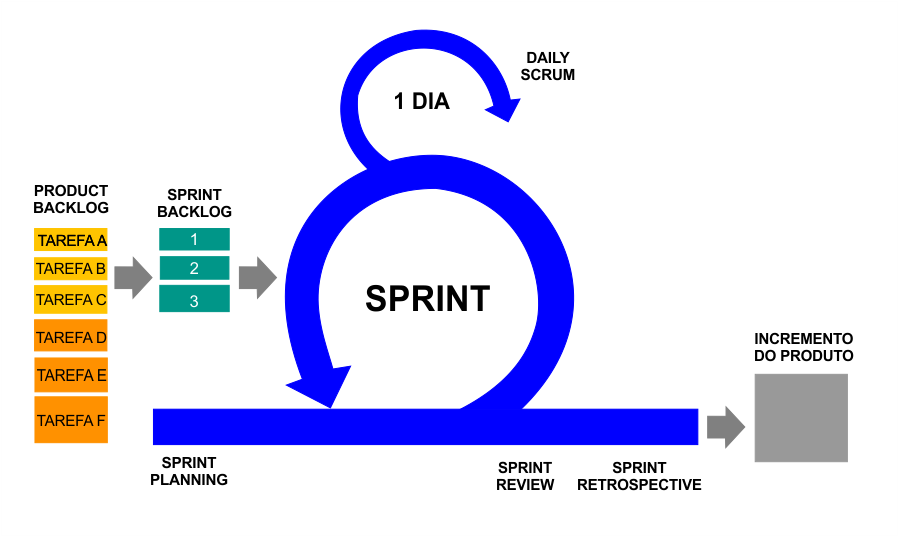
\includegraphics[scale=1.8]{Figuras/ciclo_scrum.png}
  \caption{Ciclo de atividades da metodologia \textit{Scrum}. Adaptado de \cite{0000:rafael}}
  \label{chave_para_refencia_cruzada}
\end{figure}

No decorrer do desenvolvimento vários termos são utilizados para descrever cada etapa, tais como \textit{Product Backlog, Sprint Backlog, Daily Scrum Meeting, Sprint Review Meeting,} entre outras. Adiante serão expostas cada uma com sua importância e significado dentro da metodologia.

\subsubsection{\textit{Product Backlog}}
\noindent O \textit{Product Backlog} consiste em uma lista que nela estarão elencadas tudo que acredita que será produzida ao longo do projeto e os itens presentes nela serão desenvolvidas pelo \textit{Scrum Team}, ou seja, a equipe de desenvolvimento e essa é a única fonte de trabalho que a equipe realiza. E é nela que irão conter todas a necessidades e objetivos de negócio do cliente e as partes interessadas do projeto \cite{0000:rafael}. Essa lista é categorizada com níveis de prioridades e essas prioridades são estabelecidas pelo \textit{Product Owner}.

A figura \ref{chave_para_refencia_cruzada} demonstra como é estruturada a lista de \textit{Product Backlog}, sendo organizada por prioridades. 

\begin{figure}[!htb]
  \centering 
  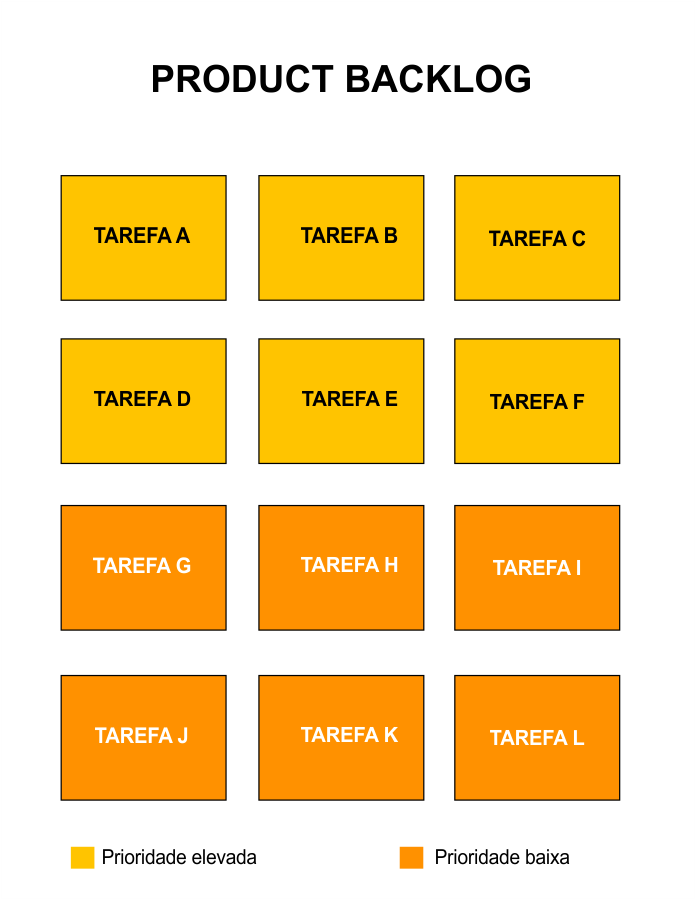
\includegraphics[scale=1.2]{Figuras/product_backlogs.png}
  \caption{Estrutura de um \textit{Product Backlog}. Adaptado de \cite{0000:rafael}}
  \label{chave_para_refencia_cruzada}
\end{figure}

\subsubsection{\textit{Sprint Backlog}}
\noindent Uma \textit{Sprint} de acordo com Kotonya \cite{1997:Kotonya} consiste em um planejamento que visa avaliar a situação do trabalho, os recursos alocados para o desenvolvimento são selecionados e o \textit{software} é implementado. Desse modo, ela é basicamente uma lista que o time de desenvolvimento se compromete a realizar as tarefas presentes. Uma \textit{Sprint} é criada no primeiro evento realizado no ciclo, que é a \textit{Sprint Planning}. Durante a \textit{Sprint} a equipe de desenvolvimento verifica o quadro e solicita a tarefa que acredita que irá conseguir desenvolver e levando em consideração as prioridades de cada.

A figura \ref{chave_para_refencia_cruzada} demonstra a estruturação de um quadro de \textit{Sprint}, sendo que é dividido em tarefas que tem para fazer, as que estão em desenvolvimento e as que já estão feitas.

\begin{figure}[!htb]
  \centering 
  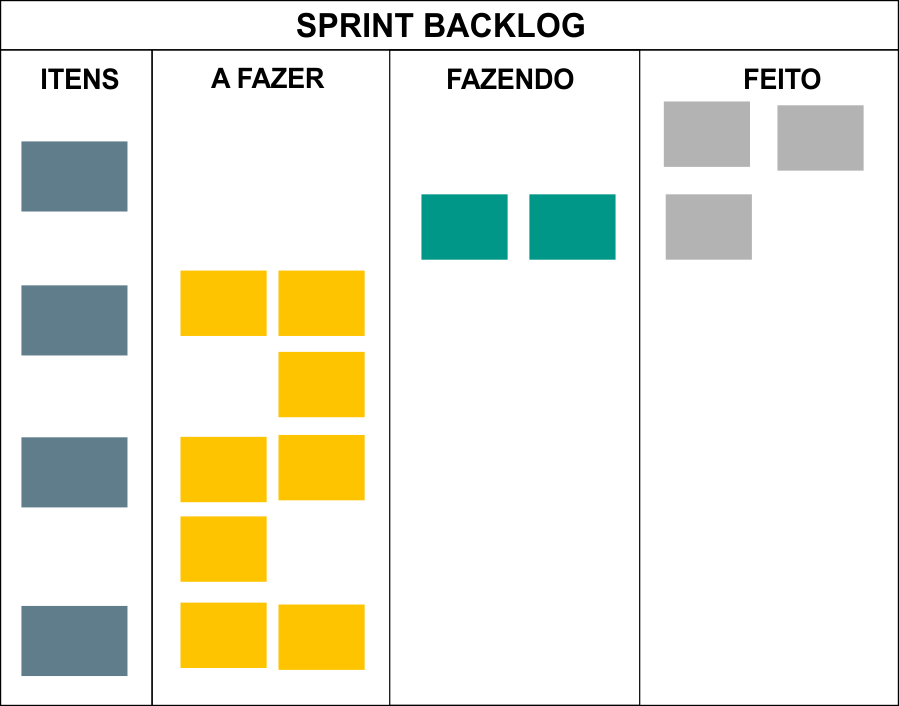
\includegraphics[scale=1.5]{Figuras/sprint_backlog.png}
  \caption{Quadro de tarefas de uma \textit{Sprint Backlog}. Adaptado de \cite{0000:rafael}}
  \label{chave_para_refencia_cruzada}
\end{figure}

\subsubsection{\textit{Daily Scrum Meeting}}
\noindent Todos os dias que os \textit{Sprints} são realizadas a equipe de desenvolvedores, \textit{Product  Owner},\textit{Scrum Master} e outras pessoas, sendo que estas só poderão escutar, participarão de uma reunião que apresenta como objetivo disseminar conhecimentos sobre o que foi realizado no dia anterior e assim conseguir identificar problemas que estão atrapalhando o desenvolvimento e nela são priorizados o trabalho que será realizado no dia.

\subsubsection{\textit{Sprint Review Meeting}}
\noindent Assim como antes de iniciar um \textit{Sprint} é realizado uma reunião para disseminação das informações, no final de cada \textit{Sprint} é realizado também uma reunião que essa apresenta como objetivo de demonstrar o que foi desenvolvido durante o dia, a qual nela participarão toda a equipe, como o \textit{Product Owner, Scrum Team, Scrum Master}, gerência, clientes e engenheiros.

\subsubsection{\textit{Product Owner}}
\noindent Esse é um dos principais personagens da metodologia \textit{Scrum}, pois ele é o responsável por garantir e maximizar o trabalho da equipe, sendo ele que define os itens que irão compor o \textit{Product Baclog}. A partir do momento em que a equipe compromete-se em desenvolver as atividades no \textit{Sprint} ele se compromete a não trazer novos requisitos para \textit{Scrum Team}.

\subsubsection{\textit{Scrum Master}}
\noindent O \textit{Scrum Master} apresenta como função dentro da metodologia de assegurar que a equipe respeite e siga os valores e práticas do \textit{Scrum}, bem como também é o responsável por resolver qualquer impedimento que venha surgir no decorrer da \textit{Sprint}.

\section{Avaliação da aprendizagem}
\noindent A prática de avaliar o aprendizado está presente em todos os momentos da vida acadêmica de um estudante, visto que essa prática faz parte dos objetivos das escolas. E a avaliação de acordo Libâneo \cite{1990:libaneo} não se restringe somente ao processo de realizar provas e atribuir notas, ela é bem mais complexa, pois tem o papel de cumprir as funções pedagógicas-didáticas que se refere ao papel da avaliação seguindo os objetivos gerais e específicos da educação escola, de diagnóstico e de controle em relação aos níveis de rendimento escolar. E esta é uma tarefa necessária e permeante do trabalho do docente. Desse modo, o autor a define como sendo uma reflexão sobre as condições de qualidade do trabalho dos dois personagens principais da academia, os professores e os alunos.

Silva \cite{2015:Silva} apresenta um conceito sobre avaliar parecido com o de Libâneo \cite{1990:libaneo} em que a avaliação não restringe somente no processo de atribuir notas ou conceito para os discentes, mas sim conseguir identificar os espaços que são deixados no decorrer do aprendizado e assim analisar e aplicar estratégias a fim suprir as necessidades identificadas.

Para Datrino \cite{2010:Datrino} na definição de avaliação existem alguns itens que são considerados elementos chaves, sendo eles: julgamento, apreciação, valoração e qualquer efeito que implicar em julgar. Apesar de avaliar implicar medição, a avaliação é algo que é bem mais abrangente do que simplesmente realizar a medição ou qualificação de alguém para saber se adquiriu os conhecimentos.

% ----------------------------------------------------------------------------------------------------- %
% Capítulo 4 - TRABALHOS RELACIONADOS
% ----------------------------------------------------------------------------------------------------- %
\chapter{Trabalhos Relacionados}
\label{cap:trabalhos}

\noindent Neste capítulo está apresentados os trabalhos correlatos com ênfase em \textit{softwares} com foco no ensino e aprendizagem, que são considerados relevantes para embasamento dessa pesquisa. As seções estão estruturas em: métodos aplicados e resultados da pesquisa.

\section{Ensino e aprendizagem de cálculo: a partir do uso de \textit{softwares} matemáticos}

\noindent A presente pesquisa de Silva e Alves \cite{2016:Santana} apresenta como objetivo analisar as supostas contribuições no ensino e aprendizagem do conceito de derivadas de uma função de uma variável real com a utilização de \textit{softwares} matemáticos.

A disciplina de Cálculo Diferencial e Integral por ser de grande importância para os cursos da área de ciências exatas e por apresentar grau de dificuldade no processo do ensino e absorção por parte dos acadêmicos, alguns métodos e estratégias são aplicadas nesse processo para facilitar o ensino e aprendizagem dos acadêmicos. Diante dessa situação, ferramentas tecnológicas como \textit{softwares} são desenvolvidos com esse objetivo e consequentemente reduz os altos índices de reprovações e evasões. 

Os autores destacam um ponto importante em relação ao processo de ensino e aprendizagem, que é a metodologia aplicada, onde a metodologia utilizada por parte dos docentes ainda persiste a tradicional, a qual essa é caracterizada pelo o ensino a partir de definições, enunciados, teoremas, demostrações e exercícios, estando restrito somente ao quadro, giz e apagador. A presente metodologia faz com que a maioria dos estudantes apenas resolvam questões aplicando fórmulas, que muitas vez são memorizadas somente para resolver durante as avaliações, o que desse modo, não compreendem nenhum dos conceitos envolvidos na resolução do problema. Mas, outra metodologia tem surgido para tentar contornar essa situação que é a com utilização de recursos tecnológicos

\subsection{Métodos Aplicados}
\noindent O estudo utilizado pelos os autores abordaram a metodologia qualitativa afim de identificar \textit{softwares} matemáticos, para isso, foi realizada a seleção de trabalhos que tratavam sobre o ensino e aprendizagem de cálculo a partir do uso de \textit{softwares} matemáticos a partir desses trabalhos selecionados os mesmos foram estudados a fim de verificar os \textit{softwares} que contribuíram para o aprendizado.

\subsection{Resultados}
\noindent Com a análise realizada pelos os autores \cite{2016:Santana} concluiu que a utilização das tecnologias estão cada vez mais presentes e seu uso está crescente nos ambientes da sociedade, especialmente na educação. Constatou também que de acordo, com a escolha de bons \textit{softwares} e aplicação de uma metodologia correta para o ensino, o uso do computador e das tecnologias presentes trazem grandes vantagens para o ensino de cálculo, pois torna o aprendizado dos discentes mais proveitoso em relação a metodologia tradicional aplicada.  

\section{Criação de um \textit{software} de apoio ao ensino e à aprendizagem de Álgebra Linear}

\noindent Na dissertação de Rodrigues \cite{2009:Rodrigues} é abordada a criação de um \textit{software} para auxiliar no ensino e à aprendizagem de base e dimensão de um espaço vetorial de uma turma de licenciatura de matemática. Segundo o autor, o alto grau de abstração dos assuntos e ao grande volume de informações torna um ponto para os altos índices de reprovações e evasões dos alunos, a partir de tal situação, surge a necessidade de uma intervenção para colaborar no ensino e aprendizagem destes conteúdos. A qual, a partir das intervenções é possível identificar recursos metodológicos para ajudar no aprendizado dos acadêmicos, um exemplo, são \textit{softwares} que são desenvolvidos para amenizar esses altos índices.

\subsection{Métodos Aplicados}
\noindent O \textit{software} foi desenvolvido em três módulos, sendo eles: introdução, base e dimensão e para a avaliação do aprendizado por parte dos estudantes foram realizadas separadamente em cada módulo. Os métodos usados para verificar o aprendizado foi avaliação heurística, questionário de satisfação e avaliação de conteúdo.

A avaliação heurística foi aplicada com objetivo de identificar problemas de usabilidade do \textit{software}, o questionário de satisfação teve como objetivo verificar o grau de satisfação do usuário quanto a abordagem do conteúdo pelo \textit{software} e para a avaliação dos conteúdos o autor aplicou duas atividades escritas e individuais a fim de identificar se os alunos conseguiram abstrair o conteúdo apresentado.

\subsection{Resultados}
\noindent De acordo com a metodologia e aplicação do \textit{software} com objetivo de verificar se o sistema conseguiria melhorar o aprendizado dos alunos de uma turma de matemática em relação aos conteúdos de Álgebra Linear. Obteve-se como resultados que a partir da utilização do \textit{software} houve melhora no aprendizado dos acadêmicos em que \cite{2009:Rodrigues} destaca que os conteúdos propostos no sistema foram compreendidos pela a maioria dos estudantes participantes. Desse modo, o autor concluiu a partir da análise dos três módulos utilizados no \textit{software} que o mesmo contribuiu para o entendimento dos conceitos.

\section{O programa GAP como ferramenta de ensino e aprendizagem de Álgebra e uma reflexão das dificuldades da disciplina Álgebra I}  

Na presente pesquisa realizada por \cite{2016:Santos} são destacados pontos importantes no que tange ao aprendizado de uma turma de alunos do curso de Licenciatura de Matemática em específico da turma de Álgebra Linear I na Universidade Federal do Goiás, a qual a motivação dos autores partiu pelos os altos índices de desistência da citada disciplina. Partindo dessa situação o objetivo do estudo foi buscar novas metodologias para auxiliar no ensino e aprendizagem dos acadêmicos.

Com o advento das ferramentas tecnológicas, trouxe consigo novas formas de aprendizados e diante, os autores explanam que essas ferramentas modificam a forma como o aprendizado acontece, visto o que antes era somente o modelo tradicional aplicado para o ensino. Onde nesse modelo consiste em uma sala de aula em que o professor possui todo o conhecimento e os alunos são passíveis no ensino e os únicos recursos para o ensino presente são somente um quadro, giz e apagador. Mas com a era das ferramentas tecnológicas esses recursos foram alterados e o aprendizado dos estudantes começaram a romper as barreiras que antes estavam restritos somente a sala de aula.

\subsection{Métodos Aplicados}
\noindent A pesquisa apresentou como enfoque investigar as vantagens da utilização de tecnologias no ensino superior com o \textit{software} GAP (\textit{Groups, Algorithms, Programming - System for Computational Discrete Algebra}) para auxiliar no aprendizado. Para a análise foi aplicados questionários e entrevistas a fim de identificar pontos chaves em relação ao aprendizado dos estudantes, ao qual esses foram aplicados antes de uma aula no modelo tradicional e logo depois outra aula já com a utilização de ferramentas tecnológicas. Quanto a utilização do \textit{software} GAP, inicialmente os pesquisadores participaram de uma aula de forma tradicional e depois os mesmos participaram e prepararam de uma já com a utilização do \textit{software} GAP com objetivo de facilitar e motivar o processo de ensino e aprendizagem na disciplina de Álgebra Linear.

\subsection{Resultados}
\noindent Com a utilização do \textit{software} GAP houve despertar, curiosidades e motivação dos alunos em relação a disciplina. E diante das análises realizadas através dos questionários e entrevistas bem como nas aulas com a utilização do GAP trouxe pontos positivos no aprendizados dos acadêmicos.
% ----------------------------------------------------------------------------------------------------- %
% Capítulo 5 - METODOLOGIA
% ----------------------------------------------------------------------------------------------------- %
\chapter{Metodologia Proposta}
\label{cap:metodologia}

\noindent No decorrer deste capítulo é descrito a aplicação das técnicas para avaliação do aprendizado dos acadêmicos da turma de Álgebra Linear do curso de Ciência da Computação da Universidade Federal do Tocantins, bem como também a Engenharia de \textit{Software} abordada no Capítulo 3 (Fundamentação Teórica) e os recursos aplicados para o desenvolvimento do \textit{software}. O objetivo desse é demonstrar as metodologias adotadas para a avaliação do aprendizado do alunos e englobando o desenvolvimento das funcionalidades do \textit{software} AlfaGebra. 

A estrutura desta capítulo está dividido em duas seções principais, sendo elas: Avaliação do aprendizado e desenvolvimento da plataforma, e nelas estão incluídos subseções que são de grande importância para o entendimento do funcionamento.

\section{Avaliação do aprendizado}
\noindent A presente pesquisa objetiva avaliar o aprendizado dos acadêmicos a partir da utilização da plataforma de ensino e aprendizagem AlfaGebra, e para esse fim, está sendo estudada a turma do período 2017-1, turma essa que não utilizará o \textit{software} AlfaGebra no decorrer do período e será também estudada a turma do período 2017-2, a qual utilizará \textit{software} no decorrer do período. Entre ambas as turmas será comparado o nível de aprendizado com o sistema, para que assim possa ser estabelecido se houve melhora no aprendizado da turma que utilizou a ferramenta ou não. É importante salientar que para as duas turmas o professor ministrante será o mesmo, tornando por conseguinte um ponto de grande importância, pois a metodologia aplicada no decorrer da turma que não utilizará o \textit{software} será a mesma com a que utilizará a ferramenta, destacando o ponto que diferencia só no quesito de utilização do sistema.

Para a metodologia de avaliação do desempenho dos acadêmicos será aplicado a pesquisa-ação, que é um método de pesquisa em campo, ao qual os dados são coletados no local em que ocorrer o problema, por meio de questionários e/ou entrevistas, mas a presente pesquisa em questão abordará a aplicação de questionários. Um ponto de destaque nessa metodologia é que ela trata de um estudo de forma qualitativa e quantitativa, pois o objetivo da avaliação é verificar melhora no aprendizado dos estudantes, pois nas etapas inciais foi realizado um estudo nos três últimos semestre a fim de identificar o quantitativo de alunos reprovados por faltas, aprovados por notas e reprovados por notas.

Para a realização desse objetivo será aplicado o método de avaliação dos acadêmicos através de coletas de dados e como instrumentos de geração de dados serão aplicados questionários de acordo com as especificações descritas a seguir:

\begin{enumerate}
    \item Questionário base - nessa etapa foi aplicado um questionário base com perguntas objetivas de múltipas escolhas e discursivas com foco em identificar o perfil dos estudantes, tais como a quantidade de vezes que o estudante está realizando a disciplina, os métodos que são aplicados para o aprendizado dos conteúdos abordados na disciplina, dificuldade encontrada na disciplina, se a aplicação de recursos tecnológicos facilitaria o aprendizado, entre outras questões relevantes, vide Apêndice II. Importante ressaltar que esse questionário foi aplicado junto a turma de Álgebra Linear que não está utilizando o \textit{software} como ferramenta de aprendizagem.
    
    \item Questionário avaliação - na presente etapa será aplicado um questionário com objetivo de identificar a melhora no aprendizado dos acadêmicos, com perguntas semelhantes a etapa anterior, tais como: a partir da utilização da plataforma houve melhora no seu aprendizado, como seria seu aprendizado sem a plataforma, entre outras perguntas. É importante destacar que o questionário será aplicado junto a turma de Álgebra Linear que estará utilizando a plataforma AlfaGebra como recursos tecnológicos para o aprendizado e nessa etapa, periodicamente, os pesquisadores estarão acompanhando os estudantes a fim de identificar pontos chaves no aprendizado.
\end{enumerate}


\section{Desenvolvimento da Plataforma}
\noindent Para o desenvolvimento da plataforma AlfaGebra algumas etapas estão sendo aplicadas para a conclusão do sistema. Inicialmente, foi desenvolvido o documento de especificações de requisitos, vide Apêndice I, ao qual de acordo com Sommerville \cite{2013:Sommerville} esse documento abrange as características do sistema, tais como o que o sistema deve fazer, as propriedades emergentes desejáveis e essenciais e as restrições quanto à operação do sistema e quanto aos processos de desenvolvimento de \textit{software}. 

Após, será realizado a prototipagem das telas, a fim de criar os esboços das telas que oferecerão suporte para o desenvolvimento do sistema. Em seguida, serão criados os diagramas de UML (\textit{Unified Modeling Language}) do sistema, que define uma série de artefatos que ajudam na tarefa de modelar e documentar o sistema orientado a objeto que será desenvolvido.

Com as etapas supracitadas concluídas, será iniciado o desenvolvimento do código fonte do \textit{software} e com a conclusão do sistema será realizado o teste de usabilidade, com objetivo de verificar junto aos usuários a facilidade que o \textit{software} apresenta ao usar. É importante enfatizar que no decorrer do desenvolvimento do sistema estarão ocorrendo testes de funcionalidades, isso nos módulos já concluídos a fim de encontrar falhas e serem corrigidas.

\subsection{Conteúdos matemáticos abordados na plataforma AlfaGebra}
\noindent Nesta seção estão descritos os conteúdos que irão ser abordados no \textit{software}, tanto para sistemas de equações lineares como espaço vetorial. Todo o conteúdo abordado segue o plano de ensino da disciplina de Álgebra Linear do curso de Ciência da Computação.  

\subsubsection{Sistemas de equações lineares:}
\begin{itemize}
    \item[1)] Operações elementares
    \item[2)] Matriz forma escada ou linha reduzida
    \item[3)] Teorema sistema de equações lineares
    \item[4)] Soluções de Sistema de n equações lineares com m variáveis
\end{itemize}

\subsubsection{Espaço Vetorial:} 
\begin{itemize}
    \item[1)] Espaços Vetoriais
    \item[2)] Propriedades dos espaços vetoriais
    \item[3)] Subespaços vetoriais
    \item[4)] Combinação linear
    \item[5)] Subespaço gerado
    \item[6)] Dependência e Independência Linear
    \item[7)] Base de um espaço vetorial
    \item[8)] Matriz de mudança de base
\end{itemize}

A plataforma apresentará material teórico sobre cada tópicos e exercícios resolvidos para que os acadêmicos possam entender todos os conceitos necessários relacionados a cada assunto. Além de todo o conteúdo teórico, o estudante poderá interagir com a mesma, onde entrará com expressão a resolvida e o sistema resolverá mostrando a descrição de como foi resolvido o problema em questão. Com essa abordagem possibilitará aos acadêmicos um aprendizado teórico, prático e dinâmico.

\subsection{Ambiente Computacional}
\noindent No decorrer desta seção são demonstrados os ambientes computacionais que serão utilizados para o desenvolvimento da plataforma de ensino e aprendizagem AlfaGebra. Para identificação das tecnologias a serem utilizadas, foi realizado um estudo junto as principais tecnologias presente no mercado que fossem \textit{open source} e que possibilitaria o desenvolvimento de um sistema flexível e que viabilizasse o gerenciamento do \textit{software} em equipe. De acordo, com a pesquisa foi escolhido como ferramenta de versionamento de código o GIT\footnote[6]{GIT \url{https://git-scm.com/}} e para hospedagem foi escolhida o sistema Bitbucket\footnote[7]{Bitbucket \url{https://bitbucket.org/product}}, devido o mesmo possibilitar a criação de repositórios remotos de acesso privados, mas é importante ressaltar que após a conclusão do AlfaGebra, o objetivo é disponibilizar o código fonte para a comunidade de programadores, visto que um dos requisitos desse sistema é que ele seja educativo e com código fonte aberto.

Para o desenvolvimento da plataforma será utilizada como arquitetura de desenvolvimento corporativa a {Plataforma Java Standard Edition} (Java SE)\footnote[8]{Java SE \url{http://www.oracle.com/technetwork/java/javase/overview/index.html}}, juntamente com a biblioteca JavaFX\footnote[9]{JavaFX \url{http://www.oracle.com/technetwork/pt/java/javafx/overview/index.html}} para a criação de interfaces gráficas agradáveis e o ambiente de desenvolvimento integrado (IDE) será adotada o Netbeans\footnote[10]{Netbeans \url{https://netbeans.org/}} para a codificação. O fluxo de programação iniciará a partir do computador de desenvolvimento, em que nele estarão instaladas as ferramentas descritas acima.

A figura \ref{fluxograma} apresenta o fluxograma de desenvolvimento do \textit{software} AlfaGebra, na qual a prototipação será a etapa de criação das telas que apresentará o sistema e as suas funcionalidades, na etapa de codificação será iniciada a implementação do sistema e em cada tarefa que será concluída de acordo com a metodologia ágil \textit{Scrum}, essa será submetida a testes, assim caso não apresente falhas, a tarefa estará concluída, mas caso o contrário irá retornar para a etapa de codificação para solucionar o problema.

\begin{figure}[!htb]
  \centering 
  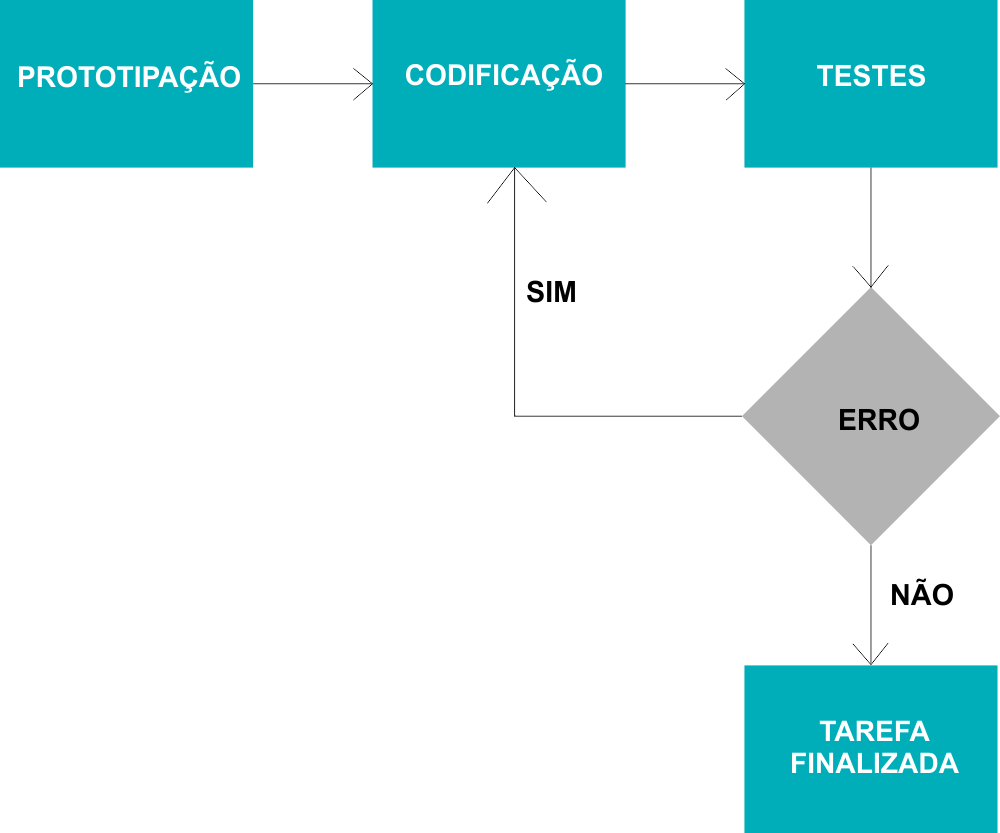
\includegraphics[scale=1]{Figuras/fluxo.png}
  \caption{Fluxo do desenvolvimento do AlfaGebra}
  \label{fluxograma}
\end{figure}

\subsection{Métodos}
\noindent Nesta seção são demonstrados os métodos a serem aplicados para o desenvolvimento da plataforma de ensino e aprendizagem AlfaGebra, com objetivo de explanar detalhadamente como ocorrerão as etapas de prototipagem das telas, aplicação da metodologia de desenvolvimento ágil \textit{Scrum} e teste de usabilidade.

\subsubsection{Prototipagem - Desenho das telas}
\noindent Para a realização da prototipagem das telas, serão desenhadas à mão, ou com \textit{software} específicos para gerar os esboços das telas e uma vez os desenhos concretizados irá oferecer suporte para os programadores no decorrer do desenvolvimento. 

\subsubsection{Desenvolvimento Ágil (\textit{Scrum})}
\noindent Com a aplicação da metodologia de desenvolvimento ágil \textit{Scrum} será possível organizar todas as tarefas de programação da plataforma AlfaGebra, de forma a ter um desenvolvimento intuitivo e organizado. Para a aplicação desta metodologia será utilizada a ferramenta de gerenciamento de projetos colaborativa, Trello\footnote[11]{Trello \url{https://trello.com}}, em virtude da mesma apresentar características como, por exemplo, de ser ajustada de acordo com as necessidades dos usuários.

Para esse projeto a estrutura de representação das tarefas serão divididas em 4 (quatro) colunas, sendo as tarefas a fazer, em desenvolvimento, finalizadas e em testes. Na coluna de tarefas a fazer serão descritas todas as tarefas que serão realizadas para a conclusão do projeto. Na tarefa em desenvolvimento são descritas todas as tarefas que foram inciadas a implementação, mas que ainda não foram concluídas, na finalizada são descritas todas as tarefas que que foram finalizadas e por fim, a coluna em testes são as tarefas que foram finalizadas, mas que estão em teste para verificar alguma falha no seu funcionamento. 

Diante das informações supracitadas todas as tarefas serão baseadas na metodologia de desenvolvimento ágil \textit{Scrum}, a partir do conceito dos \textit{backlog} e das demandas a serem entregas a partir das definições dos \textit{sprints} e o acompanhamento do projeto será realizado periodicamente em reuniões com a equipe do projeto.

\subsubsection{Teste de Usabilidade}
\noindent Em virtude da avaliação do resultado final do \textit{software}, no presente trabalho será aplicado o teste de usabilidade a fim de identificar a performance alcançada pelos usuários e o entendimento das funções do sistema. Visto que uma interface com boa usabilidade possibilita que o usuário torne-se mais produtivo, em virtude em que ele não irá interromper o processo para buscar orientação quanto alguma dúvida do sistema.

Para a concretização do teste será aplicado um questionário, que abrangerá afirmativas com as possibilidades de excelente, ótimo, bom, regular e péssima, junto aos alunos da disciplina de Álgebra Linear do curso de Ciência da Computação que utilizaram o sistema no decorrer do semestre 2017-2 e assim identificar pontos positivos e negativos do sistema e buscar solucionar os negativos em atualizações futuras. 

\begin{comment}
\subsection{Diagramas UML}
\noindent

\subsubsection{Diagrama de Caso de Uso}
\noindent

\subsubsection{Diagrama de Classe}
\noindent

\subsubsection{Diagrama de Atividade}
\noindent

\subsubsection{Diagrama de Implementação}
\noindent
\end{comment}

\subsection{Ferramentas e Materiais}
\noindent Nesta seção são descritas as ferramentas tecnológicas utilizadas para a construção da plataforma de ensino e aprendizagem AlfaGebra. A seguir estão descritos todos os recursos tecnológicos que serão aplicados para que a plataforma possa ser concretizada.

\begin{itemize}
    \item \textit{Plataforma Java Standard Edition} (Java SE)\footnote[12]{Java SE \url{http://www.oracle.com/technetwork/java/javase/overview/index.html}}
\end{itemize}
\noindent A presente plataforma é uma ferramenta para desenvolvimento de \textit{software}, que permite desenvolver e implementar aplicativos Java em \textit{desktops} e servidores. a Java SE é mantida pela empresa Sun Oracle para a comunidade de programadores Java.

\begin{itemize}
    \item JavaFX \textit{Sciene Builder}\footnote[13]{JavaFX \url{http://www.oracle.com/technetwork/pt/java/javafx/overview/index.html}}
\end{itemize}
\noindent JavaFX é uma conjunto de pacotes gráficos e de mídia que possibilita aos programadores criar, testar, depurar e implementar aplicações. Lançada pela a Sun Oracle para a criação de aplicativos para diversas plataformas como \textit{desktop}, web, \textit{mobile}, etc., ela conta com recursos para personalizar a aparência das aplicações, tais como folha de estilos em cascata (CSS), recursos bastante utilizados em desenvolvimento web para personalizar a aparência das aplicações. A escolha dessa biblioteca foi devido às informações supracitadas e que o objetivo é desenvolver uma plataforma com \textit{interface} bem agradável para o usuário.

\begin{itemize}
    \item Netbeans IDE\footnote[14]{Netbeans \url{https://netbeans.org/}}
\end{itemize}
A IDE utilizada para o desenvolvimento do \textit{software} em versão para \textit{desktop} será Netbeans, que oferece suporte de primeira classe para as tecnologias e melhorias de especificações Java mais recentes. Sua escolha foi realizada pela a equipe de desenvolvimento devido a mesma apresentar amplo suporte à criação de aplicações Java e por ser gratuita.

\begin{itemize}
    \item PrimeFaces\footnote[15]{PrimeFaces \url{https://www.primefaces.org/}}
\end{itemize}
Primefaces é um \textit{framework} \textit{openSource} de componentes para Java, que apresenta como objetivo fornecer componentes padrões para \textit{Java Server Faces}. Apesar de sua aplicação ser voltada para desenvolvimento web este estará sendo utilizado para desenvolvimento \textit{desktop}. A escolha dessa ferramenta foi realizada para a geração de gráficos, em virtude da plataforma AlfaGebra irá apresentar, sempre que possível, a interpretação geométrica, de forma a dinamizar, simplificar e otimizar o conhecimento.

\begin{itemize}
    \item iText\footnote[16]{iText \url{https://itextpdf.com}}
\end{itemize}
O iText é um conjunto de ferramentas \textit{open source} desenvolvido para a comunidade de desenvolvedores de \textit{software}, que permite a integração de funcionalidades em PDF \textit{Portable Document Format} (Formato Portátil de Documento) nas aplicações. A sua escolha foi aplicada devido a necessidade de gerar arquivos PDF na plataforma para que os acadêmicos possam ter esse recurso a sua disposição, por exemplo, na resolução de uma determinada questão.

É provável que alguns itens apresentados nesse projeto venham a sofrer alterações no decorrer da execução do desenvolvimento da plataforma, pois na medida que é iniciado o estudo e desenvolvimento, melhores ferramentas podem ser adotas para facilitar o processo. Assim como, poderá ser adicionados novas ferramentas de acordo com as necessidades de desenvolvimento.
% ----------------------------------------------------------------------------------------------------- %
% Capítulo 6 - RESULTADOS
% ----------------------------------------------------------------------------------------------------- %
\chapter{Resultados Preliminares}
\label{cap:resultados}
\noindent No presente capítulo são descritos os resultados parciais qualitativos e quantitativos obtidos no decorrer da aplicação do questionário de avaliação do aprendizado dos estudantes da disciplina de Álgebra Linear que não estão utilizando a plataforma AlfaGebra.

\section{Disciplina Álgebra Linear}
\label{disciplina_3_ultimos_semestre}

\noindent Dados fornecidos pela professora da disciplina de Álgebra Linear, mostram que existem uma percentagem muito elevada de alunos evadidos no decorrer de cada semestre. Obtendo como base os três últimos semestre, 2015-2, 2016-1 e 2016-2, observa-se um número elevado de alunos que são reprovados por faltas como demonstrado na tabela \ref{dados_tres_semestres_alunos_algebra} que além de demonstrar os reprovados por faltas, mostra também a quantidade dos que foram aprovados por notas e reprovados por notas. É importante salientar que conforme a professora da disciplina, os acadêmicos já começam a evadir, logo após a aplicação da primeira avaliação. Estabelecendo uma média em relação a esses semestres, apresenta-se uma porcentagem de aproximadamente 47,06\% de alunos que são evadidos da disciplina, um dado que corresponde a quase metade dos alunos.
\begin{table}[!htp]
    \centering
    \begin{tabular}{lcccl}
                                                                            & \multicolumn{1}{l}{}                                         & \multicolumn{1}{l}{}                                         & \multicolumn{1}{l}{}                                         &  \\
                                                                            & \multicolumn{1}{l}{}                                         & \multicolumn{1}{l}{}                                         & \multicolumn{1}{l}{}                                         &  \\ \cline{1-4}
\multicolumn{1}{|l|}{}                                                      & \multicolumn{3}{c|}{\textbf{PERÍODO}}                                                                                                                                                      &  \\ \cline{2-4}
\multicolumn{1}{|l|}{\multirow{-2}{*}{}}                                    & \multicolumn{1}{c|}{\cellcolor[HTML]{EFEFEF}\textbf{2015-2}} & \multicolumn{1}{c|}{\cellcolor[HTML]{EFEFEF}\textbf{2016-1}} & \multicolumn{1}{c|}{\cellcolor[HTML]{EFEFEF}\textbf{2016-2}} &  \\ \cline{1-4}
\multicolumn{1}{|c|}{\textbf{Matriculados}}                                 & \multicolumn{1}{c|}{38}                                      & \multicolumn{1}{c|}{40}                                      & \multicolumn{1}{c|}{41}                                      &  \\ \cline{1-4}
\multicolumn{1}{|c|}{\cellcolor[HTML]{EFEFEF}\textbf{Aprovados}}            & \multicolumn{1}{c|}{\cellcolor[HTML]{EFEFEF}10}              & \multicolumn{1}{c|}{\cellcolor[HTML]{EFEFEF}20}              & \multicolumn{1}{c|}{\cellcolor[HTML]{EFEFEF}15}              &  \\ \cline{1-4}
\multicolumn{1}{|c|}{\textbf{Reprovados por faltas}}                        & \multicolumn{1}{c|}{21}                                      & \multicolumn{1}{c|}{12}                                      & \multicolumn{1}{c|}{23}                                      &  \\ \cline{1-4}
\multicolumn{1}{|c|}{\cellcolor[HTML]{EFEFEF}\textbf{Reprovados por notas}} & \multicolumn{1}{c|}{\cellcolor[HTML]{EFEFEF}7}               & \multicolumn{1}{c|}{\cellcolor[HTML]{EFEFEF}8}               & \multicolumn{1}{c|}{\cellcolor[HTML]{EFEFEF}3}               &  \\ \cline{1-4}
\end{tabular}
    \caption{Dados dos quantitativos de alunos nos três últimos semestres, referentes a aprovados por notas, reprovados por faltas e reprovados por notas}
    \label{dados_tres_semestres_alunos_algebra}
\end{table}

A tabela \ref{algebra_linear_2015_2} demonstra os resultados da disciplina de Álgebra Linear no semestre de 2015-2, em relação ao quantitativo de alunos que foram aprovados, reprovados por faltas e reprovados por notas, ao qual nesse período a citada disciplina apresentava um total de 38 alunos e dentre esses, apenas 26,32\% foram os aprovados por notas, 55,26\% reprovados por faltas e 18,42\% reprovados por notas.

\begin{figure}[!htb]
  \centering 
  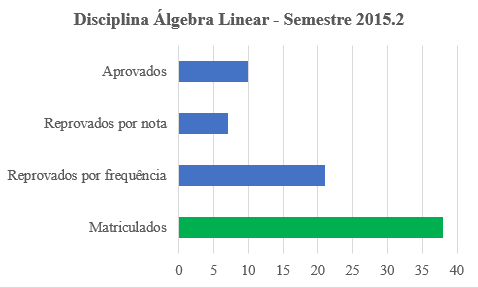
\includegraphics[scale=1]{Figuras/2015-2.png}
  \caption{Dados dos alunos referente a disciplina de Álgebra Linear no semestre 2015-2}\label{algebra_linear_2015_2}
\end{figure}

Em relação ao semestre de 2016-1, na figura \ref{algebra_linear_2016_1} são destacados o quantitativo referente ao semestre em questão, em que dentre as 3 (três) categorias, aprovados, reprovados por notas e reprovados por faltas, são destacados os seguintes dados obtidos perante a análise do gráfico: aprovados por notas cerca de 50\%, reprovados por notas 20\% e reprovados por faltas 30\%.

\begin{figure}[!htb]
  \centering 
  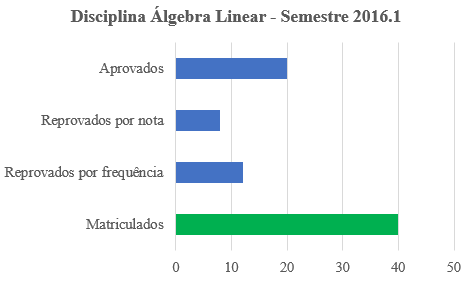
\includegraphics[scale=1]{Figuras/2016-1.png}
  \caption{Dados dos alunos referente a disciplina de Álgebra Linear no semestre 2016-1}\label{algebra_linear_2016_1}
\end{figure}

Por fim, no semestre de 2016-2, a figura \ref{algebra_linear_2016_2} mostra que mais da metade dos estudantes ficaram como reprovados por faltas, sendo 56,10\% e os demais referem-se aos reprovados por notas com um total de 7,32\% e aprovados por notas com 36,58\%.

\begin{figure}[!htb]
  \centering 
  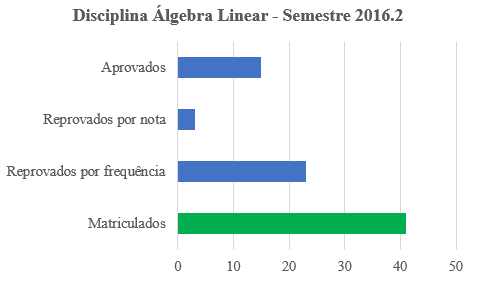
\includegraphics[scale=1]{Figuras/2016-2.png}
  \caption{Dados dos alunos referente a disciplina de Álgebra Linear no semestre 2016-2}\label{algebra_linear_2016_2}
\end{figure}

A partir desses dados é possível verificar que os índices de reprovações da disciplina nos três últimos semestres correspondem a 16,51\% e esse dado não é tão elevado, mas considerando o total de 51,37\% referente aos reprovados por faltas, esses dados poderiam ser diferentes devido ao alto nível de abstração que a disciplina apresenta, por conseguinte, muitos deles desistem.

\section{Coleta de dados}
\label{coleta_dados}

\noindent Com objetivo de investigar por que os acadêmicos da disciplina de Álgebra Linear sentem desmotivados no estudo da Álgebra Linear, as dificuldades encontradas em absorver os conteúdos da disciplina e a importância da aplicação de recursos tecnológicos para o aprendizado foi desenvolvido um questionário base estruturado como previsto na metodologia e aplicado para a turma de Álgebra Linear do semestre de 2017-1, no curso de Ciência da Computação, o qual foi aplicado no dia 19 de outubro de 2017 e apresentava perguntas objetivas de múltiplas escolhas e discursivas. A aplicação foi direcionada para um total de 40 alunos, em conformidade com o número de matriculados na disciplina, mas no dia da aplicação encontravam-se somente 22 (vinte e dois) acadêmicos presente na sala de aula e é importante salientar que já havia sido aplicada a primeira avaliação.  

Com o questionário foi possível identificar o grau de dificuldade da disciplina de acordo com os acadêmicos, a qual a figura \ref{grau_dificuldade} explana os dados obtidos e que de um total de 22 alunos que participaram da pesquisa 40,90\% consideraram a disciplina com grau de dificuldade alto, 50\% como médio, 9,10\% sendo razoável e nenhum estudante achou a disciplina fácil e os estudantes relataram que dentre os conteúdos presente na estrutura curricular da disciplina o mais difícil de absorver é espaço vetorial. Um ponto a destacar é que alguns alunos chegam no ensino superior muitas vezes despreparados em alguns assuntos da matemática o que muitas vezes torna um ponto difícil no início do estudo da Álgebra Linear e não somente nela mais também nas demais disciplinas de cálculos.

\begin{figure}[!htb]
  \centering 
  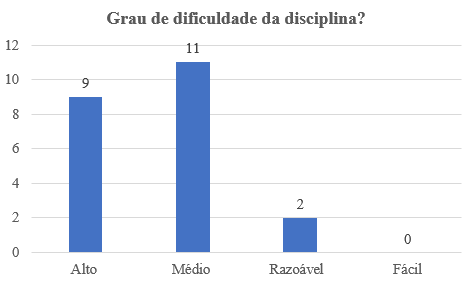
\includegraphics[scale=1]{Figuras/grau_dificuldade.png}
  \caption{Grau de dificuldade dos alunos}\label{grau_dificuldade}
\end{figure}
 
Diante dos resultados demonstrados referente ao grau de dificuldade, buscou-se entender qual é a maior dificuldade no aprendizado da Álgebra Linear e cerca de 45,45\% dos estudantes relataram que a maior dificuldade encontrada é em relação o alto nível de abstração, e para contornar esse alto nível, os acadêmicos utilizam como métodos de estudo, listas de exercícios e a maioria gosta de estudar individualmente. Vale salientar que a assiduidade com que os acadêmicos procuram o professor para sanar suas dúvidas relativas à disciplina é ínfima, a figura \ref{frequencia_procura_professor} evidencia esse dados, sendo que apenas 4,54\% dos estudantes já o procuraram nesse semestre, em condição razoavelmente, 36,36\% procuram às vezes e 54,54\% nunca procuraram.

\begin{figure}[!htb]
  \centering 
  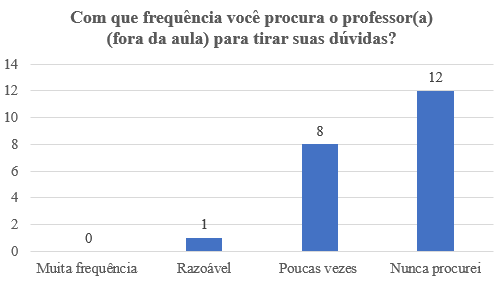
\includegraphics[scale=1]{Figuras/frequencia_professor.png}
  \caption{Frequência que os alunos procuram o professor}\label{frequencia_procura_professor}
\end{figure}

Um dado importante a ser destacado é a quantidade de vezes que o estudante está realizando a disciplina, pois este remete aos índices de reprovações e o grau de dificuldade enfrentado durante o estudo. Para esse dado, a figura \ref{numero_alunos_cursaram_vezes} mostra que 31,81\% estão realizando pela a segunda vez e 9,10\% pela terceira vez.

\begin{figure}[!htb]
  \centering 
  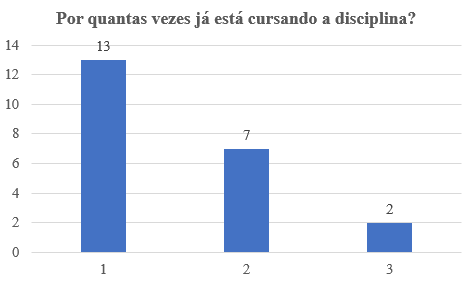
\includegraphics[scale=1]{Figuras/cursada_vezes.png}
  \caption{Quantitativo de alunos que cursaram a disciplina de Álgebra Linear}\label{numero_alunos_cursaram_vezes}
\end{figure}

Em relação ao uso de tecnologias para auxiliar no aprendizado dos conteúdos, 81,81\% dos estudantes relataram que se fosse disponibilizado algum recurso tecnológico para auxiliar no estudo/aprendizado da Álgebra Linear eles utilizariam, além dos estudantes que relataram que a utilizaria, nenhum estudante comentou que a não utilizaria, mas 18,18\% ficaram indecisos na escolha se a utilizaria ou não. Contudo, demonstraram que a ideia desse recurso tecnológico é excelente, pois ajudaria a entender os conteúdos e que seria uma nova metodologia tecnológica, na figura \ref{tecnologia_estudo} esses dados estão representados graficamente. 

No que concerne a utilização do sistema AlfaGebra, 100\% dos alunos responderam que utilizariam no decorrer dos estudos e seria uma ferramenta útil para o aprendizado e que 86,36\% relataram que a utilização desse sistema no decorrer das aulas possibilitaria maior dinamismo.

\begin{figure}[!htb]
  \centering 
  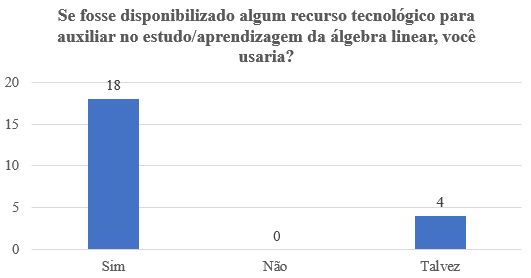
\includegraphics[scale=1]{Figuras/tecnologia_usa.png}
  \caption{Utilização de tecnologias para o estudo}
  \label{tecnologia_estudo}
\end{figure}


% ----------------------------------------------------------------------------------------------------- %
% Capítulo 6 - CONCLUSÃO
% ----------------------------------------------------------------------------------------------------- %
\chapter{Conclusões}
\label{cap:conclusoes}

\noindent As aplicações da Álgebra Linear está presente em diversas áreas e na computação não é diferente, devido a sua aplicação na computação é necessário que o estudante de um curso dessa área tenha que aprender os conceitos e métodos da Álgebra Linear para aplicá-los em problemas, mas muitos estudantes relatam que essa área é bastante difícil. Contudo, atualmente na era tecnológica alguns recursos tecnológicos são aplicados a fim de ajudar na compreensão dos assuntos, seja na Álgebra Linear ou não.

No presente trabalho demonstra conceitos e métodos para o desenvolvimento de uma plataforma de ensino e aprendizagem, com objetivo de auxiliar os acadêmicos no aprendizado dos conteúdos da disciplina de Álgebra Linear do curso de Ciência da Computação e para verificar se o \textit{software} irá auxiliar na aprendizagem dos acadêmicos será realizada uma comparação entre duas turnas de Álgebra Linear, uma correspondente ao semestre de 2017-1 e 2017-2, ao qual a de 2017-1 os acadêmicos não irão utilizar o \textit{software} AlfaGebra e no de 2017-2 os estudante irão utilizar o sistema.

A disciplina de Álgebra Linear no curso de Ciência da Computação apresenta altos índices de evasão da disciplina, bem como também reprovações, por tal motivo é proposto nesse trabalho a inserção do \textit{software} AlfaGebra para motivar os alunos no processo de ensino e aprendizagem da disciplina de Álgebra Linear.

Portanto, espera que com a aplicação da plataforma de ensino e aprendizagem AlfaGebra possa contribuir para o aprendizado dos acadêmicos. No atual momento já foi possível identificar os aspectos referente ao aprendizado e dificuldades dos estudantes a partir da aplicação do questionário base junto a turna do período de 2017-1 para assim compreender as necessidades e pontos fortes e fracos que influência na aquisição de conhecimento.


\backmatter 
\singlespacing   
% ----------------------------------------------------------------------------------------------------- %
% Bibliografia
% ----------------------------------------------------------------------------------------------------- %

\bibliography{tcc_1}

% ----------------------------------------------------------------------------------------------------- %
% Anexos
% ----------------------------------------------------------------------------------------------------- %
\appendix
% ----------------------------------------------------------------------------------------------------- %
% Apêndice 
% ----------------------------------------------------------------------------------------------------- %
\chapter{Apêndice}
\label{cap:apendice}


\section*{Apêndice I}
\label{apendice_especificacao_requisitos}
\newpage

\hline



\newpage

\section*{Apêndice II}

\subsection*{Formulário de avaliação de desempenho}
\label{questionario_base}

\begin{enumerate}
    \item Qual foi a sua maior dificuldade com a disciplina? 
    
(   ) Falta de tempo para dedicação ao estudo\\
(   ) Falta de clareza do professor\\
(   ) Desprovimento de disciplinas pré-requisitos \\
(   ) Falta de interação com professor\\
(   ) Alto nível de abstração da disciplina\\
(   ) Não consegui entender a matéria\\
(   ) Outras

    \item Por quantas vezes já está cursando a disciplina?

(   )  1 vez\\
(   )  2 vezes\\
(   )  3 ou mais

    \item Qual o método de estudo utilizado?
    
(   ) Estudo em grupo\\
(   ) Estudo através de listas de exercícios\\
(   ) Sanar dúvidas em atendimentos com professor\\
(   ) Estudo individual\\
(   ) Estudo através de livros\\
(   ) Sanar dúvidas na sala de aula\\
(   ) Outros

\item Se fosse disponibilizado algum recurso tecnológico para auxiliar no estudo/aprendizagem da álgebra linear, você usaria?

(   ) Sim\\
(   ) Não\\
(   ) Talvez

\item O que você achou da ideia de um recurso tecnológico para auxiliar no estudo/aprendizado?

(   ) Excelente\\
(   ) Boa\\
(   ) Razoável\\
(   ) Ruim\\
(   ) Péssima
	
\item Quais conteúdos gostaria que fossem abordados nesses recursos tecnológico? OBS: Pode marcar mais de um item.

(  ) Sistemas de equações Lineares\\
(  ) Espaços Vetoriais\\
(  ) Transformações lineares
	
\item Como você classifica seu aprendizado na disciplina de Álgebra Linear até o presente momento?

(   ) Excelente\\
(   ) Bom\\
(   ) Regular\\
(   ) Ruim\\
(   ) Péssimo

\item Em relação ao seu curso, você considera que essa disciplina é:

(   ) Importante\\
(   ) Tem alguma importância\\
(   ) Pouco importante

\item Qual o grau de dificuldade da disciplina?

(   ) Alto\\
(   ) Médio\\
(   ) Razoável\\
(   ) Fácil

\item Com que frequência você procura o professor(a) (fora da aula) para tirar suas dúvidas?

(   ) Muita frequência\\
(   ) Razoável\\
(   ) Poucas\\
(   ) Nunca procurei

\item Após cursar a disciplina, seu interesse pelo assunto aumentou? (Para aqueles que já cursaram mais de um vez a disciplina)

(   ) Sim\\
(   ) Não

\item Cite um ou mais pontos fortes da disciplina.

\_\_\_\_\_\_\_\_\_\_\_\_\_\_\_\_\_\_\_\_\_\_\_\_\_\_\_\_\_\_\_\_\_\_\_\_\_\_\_\_\_\_\_\_\_\_\_\_\_\_\_\_\_\_\_\_\_\_\_\_\_\_\_\_\_\_\_\_\_\_\_\_\_\_\_\_\_\_\_\_\_\_\_\_\_\_\_\_\_\_\_\_\_\_\_\_\_\_\_\_\_\_\_\_\_\_\_\_\_\_\_\_\_\_\_\_\_\_\_\_\_\_\_\_\_\_\_\_\_\_\_\_\_\_\_\_\_\_\_\_\_\_\_\_\_\_\_\_\_\_\_\_\_\_\_\_\_\_\_\_\_\_\_\_\_\_\_\_\_\_\_\_\_\_\_\_

\item Que sugestões você daria para melhorar a disciplina?

\_\_\_\_\_\_\_\_\_\_\_\_\_\_\_\_\_\_\_\_\_\_\_\_\_\_\_\_\_\_\_\_\_\_\_\_\_\_\_\_\_\_\_\_\_\_\_\_\_\_\_\_\_\_\_\_\_\_\_\_\_\_\_\_\_\_\_\_\_\_\_\_\_\_\_\_\_\_\_\_\_\_\_\_\_\_\_\_\_\_\_\_\_\_\_\_\_\_\_\_\_\_\_\_\_\_\_\_\_\_\_\_\_\_\_\_\_\_\_\_\_\_\_\_\_\_\_\_\_\_\_\_\_\_\_\_\_\_\_\_\_\_\_\_\_\_\_\_\_\_\_\_\_\_\_\_\_\_\_\_\_\_\_\_\_\_\_\_\_\_\_\_\_\_\_\_

\item Quais suas dificuldades ao estudar álgebra linear?

\_\_\_\_\_\_\_\_\_\_\_\_\_\_\_\_\_\_\_\_\_\_\_\_\_\_\_\_\_\_\_\_\_\_\_\_\_\_\_\_\_\_\_\_\_\_\_\_\_\_\_\_\_\_\_\_\_\_\_\_\_\_\_\_\_\_\_\_\_\_\_\_\_\_\_\_\_\_\_\_\_\_\_\_\_\_\_\_\_\_\_\_\_\_\_\_\_\_\_\_\_\_\_\_\_\_\_\_\_\_\_\_\_\_\_\_\_\_\_\_\_\_\_\_\_\_\_\_\_\_\_\_\_\_\_\_\_\_\_\_\_\_\_\_\_\_\_\_\_\_\_\_\_\_\_\_\_\_\_\_\_\_\_\_\_\_\_\_\_\_\_\_\_\_\_\_

\item O que você considera mais difícil na álgebra Linear? 

\_\_\_\_\_\_\_\_\_\_\_\_\_\_\_\_\_\_\_\_\_\_\_\_\_\_\_\_\_\_\_\_\_\_\_\_\_\_\_\_\_\_\_\_\_\_\_\_\_\_\_\_\_\_\_\_\_\_\_\_\_\_\_\_\_\_\_\_\_\_\_\_\_\_\_\_\_\_\_\_\_\_\_\_\_\_\_\_\_\_\_\_\_\_\_\_\_\_\_\_\_\_\_\_\_\_\_\_\_\_\_\_\_\_\_\_\_\_\_\_\_\_\_\_\_\_\_\_\_\_\_\_\_\_\_\_\_\_\_\_\_\_\_\_\_\_\_\_\_\_\_\_\_\_\_\_\_\_\_\_\_\_\_\_\_\_\_\_\_\_\_\_\_\_\_\_

\item Você conhece ou já fez uso de algum sistema que te auxiliou no estudo da álgebra linear? 

\_\_\_\_\_\_\_\_\_\_\_\_\_\_\_\_\_\_\_\_\_\_\_\_\_\_\_\_\_\_\_\_\_\_\_\_\_\_\_\_\_\_\_\_\_\_\_\_\_\_\_\_\_\_\_\_\_\_\_\_\_\_\_\_\_\_\_\_\_\_\_\_\_\_\_\_\_\_\_\_\_\_\_\_\_\_\_

\item Se sim, qual(is)?

\_\_\_\_\_\_\_\_\_\_\_\_\_\_\_\_\_\_\_\_\_\_\_\_\_\_\_\_\_\_\_\_\_\_\_\_\_\_\_\_\_\_\_\_\_\_\_\_\_\_\_\_\_\_\_\_\_\_\_\_\_\_\_\_\_\_\_\_\_\_\_\_\_\_\_\_\_\_\_\_\_\_\_\_\_\_\_\_\_\_\_\_\_\_\_\_\_\_\_\_\_\_\_\_\_\_\_\_\_\_\_\_\_\_\_\_\_\_\_\_\_\_\_\_\_\_\_\_\_\_\_\_\_\_\_\_\_\_\_\_\_\_\_\_\_\_\_\_\_\_\_\_\_\_\_\_\_\_\_\_\_\_\_\_\_\_\_\_\_\_\_\_\_\_\_\_

\item Quais os recursos (seja eles tecnológicos ou não) que o seu professor utilizou para o ensino da disciplina?

\_\_\_\_\_\_\_\_\_\_\_\_\_\_\_\_\_\_\_\_\_\_\_\_\_\_\_\_\_\_\_\_\_\_\_\_\_\_\_\_\_\_\_\_\_\_\_\_\_\_\_\_\_\_\_\_\_\_\_\_\_\_\_\_\_\_\_\_\_\_\_\_\_\_\_\_\_\_\_\_\_\_\_\_\_\_\_\_\_\_\_\_\_\_\_\_\_\_\_\_\_\_\_\_\_\_\_\_\_\_\_\_\_\_\_\_\_\_\_\_\_\_\_\_\_\_\_\_\_\_\_\_\_\_\_\_\_\_\_\_\_\_\_\_\_\_\_\_\_\_\_\_\_\_\_\_\_\_\_\_\_\_\_\_\_\_\_\_\_\_\_\_\_\_\_\_

\item Se fosse desenvolvido um sistema para auxiliar você aluno, no aprendizado da Álgebra Linear, a qual esse apresentaria um tutorial dos principais conteúdos da Álgebra e opção em que o aluno entre com a expressão e o sistema mostre o passa-a-passo da resolução. Marque o quanto ele ajudaria?

(   ) Ajudaria muito\\
(   ) Ajudaria, mas prefiro não utilizar\\
(   ) Ajudaria Pouco\\
(   ) Não ajudaria 

\item Em sua opinião a utilização desse sistema durante as aulas ou fora possibilitará mais dinamismo e aprendizado da matéria?

(   ) Sim\\
(   ) Não\\
(   ) Não sei

\end{enumerate}


%% ----------------------------------------------------------------------------------------------------- %
% Anexo
% ----------------------------------------------------------------------------------------------------- %
\chapter{Anexo}
\label{cap:anexo}
\onehalfspacing

\end{document}


